% =====================================================================
%  Chapter 4: Curves, Coordinates, and Surfaces Before Calculus
% =====================================================================

\chapter{Curves, Coordinates, and Surfaces Before Calculus}
\label{ch:4}

Chapter 3 ended with the simplest kind of nonlinear object: a curve
\[
    \mathbf r(t).
\]
A curve is a moving point.  If we later differentiate it, its derivative will be a
velocity vector.  If we later integrate along it, it will become a path that can collect
length, work, circulation, or a \(1\)-form.

Before calculus starts doing things to curves and surfaces, we need to know how to
describe them.

\section{Parametric curves}
\label{sec:4.1}

A graph like
\[
    y=f(x)
\]
describes a curve by using \(x\) as the input.  That works well for many curves, but it
is not how a moving object usually reports its position.  A boat, a drone, a planet, and
a particle do not usually say, ``here is my \(y\)-coordinate as a function of my
\(x\)-coordinate.''  They say where they are at each time.

That is the idea of a parametric curve.

\subsection{Curves as moving points}

Imagine an ant walking around the rim of a circular fountain of radius \(3\).  Put the
center of the fountain at the origin.  At time \(t\), measured in radians, suppose the
ant is at
\[
    \mathbf r(t)=(3\cos t,3\sin t).
\]
A few times give:
\[
\begin{array}{c|c}
t & \mathbf r(t) \\ \hline
0 & (3,0)\\
\dfrac{\pi}{2} & (0,3)\\
\pi & (-3,0)\\
\dfrac{3\pi}{2} & (0,-3)\\
2\pi & (3,0)
\end{array}
\]
The point moves counterclockwise and returns to where it started.

\begin{figure}[h]
\centering
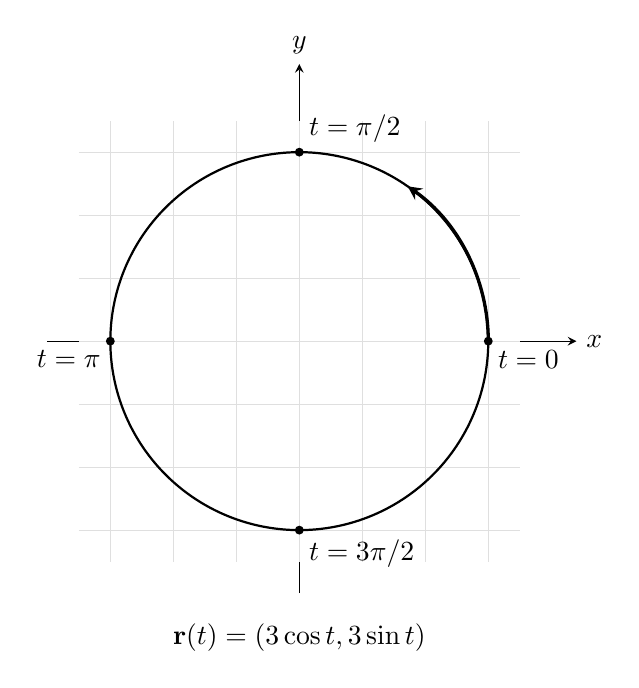
\begin{tikzpicture}[scale=0.8, >=stealth]
    \draw[->] (-4,0) -- (4.4,0) node[right] {\(x\)};
    \draw[->] (0,-4) -- (0,4.4) node[above] {\(y\)};

    \draw[gray!25, step=1] (-3.5,-3.5) grid (3.5,3.5);

    \draw[thick, domain=0:6.283, samples=160, smooth, variable=\t]
        plot ({3*cos(\t r)}, {3*sin(\t r)});

    \draw[->, very thick] (3,0) arc[start angle=0,end angle=55,radius=3];

    \fill (3,0) circle (2pt);
    \fill (0,3) circle (2pt);
    \fill (-3,0) circle (2pt);
    \fill (0,-3) circle (2pt);

    \node[below right] at (3,0) {\(t=0\)};
    \node[above right] at (0,3) {\(t=\pi/2\)};
    \node[below left] at (-3,0) {\(t=\pi\)};
    \node[below right] at (0,-3) {\(t=3\pi/2\)};

    \node at (0,-4.7) {\(\mathbf r(t)=(3\cos t,3\sin t)\)};
\end{tikzpicture}
\caption{A parametrization of a circle records a moving point, not just a set of points.}
\end{figure}

The coordinates satisfy
\[
    x=3\cos t,\qquad y=3\sin t.
\]
Using
\[
    \cos^2t+\sin^2t=1,
\]
we get
\[
    x^2+y^2=9.
\]
So the image is the circle of radius \(3\).  But the parametrization gives more
information than the equation \(x^2+y^2=9\).  It tells us where the ant starts, which
direction it walks, and how the point is traced.

\begin{definition}[Parametric curve]
A \emph{parametric curve} in \(\mathbb R^n\) is a function
\[
    \mathbf r:I\to\mathbb R^n,
\]
where \(I\) is an interval of real numbers.  The input is called the
\emph{parameter}.  Usually we write it as \(t\).

In the plane,
\[
    \mathbf r(t)=(x(t),y(t)).
\]
In space,
\[
    \mathbf r(t)=(x(t),y(t),z(t)).
\]

The \emph{image} of the curve is the set of points
\[
    \{\mathbf r(t):t\in I\}.
\]
\end{definition}

The parameter often represents time, but it does not have to.  It might represent an
angle, a distance along a track, or simply a label that tells us where we are on the
curve.

There is one quiet condition we usually want: the coordinate functions should be
continuous.  A curve should not teleport.

\begin{example}[Why continuity matters]
Define
\[
    \mathbf r(t)=
    \begin{cases}
    (0,0), & t<0,\\
    (1,0), & t\ge 0.
    \end{cases}
\]
This rule gives a point for every \(t\), but it does not describe a continuous motion.
At \(t=0\), the point jumps from \((0,0)\) to \((1,0)\).

So when we speak of a curve as a moving point, we usually mean that the component
functions are continuous.  Later, when we want velocity, we will ask for differentiability
as well.
\end{example}

\subsection{Plane curves and space curves}

A plane curve has two coordinate functions.  A space curve has three.

\begin{example}[A line segment as a parametric curve]
The straight path from
\[
    P=(1,2)
\]
to
\[
    Q=(5,4)
\]
can be written as
\[
    \mathbf r(t)=P+t(Q-P),\qquad 0\le t\le1.
\]
Since
\[
    Q-P=(4,2),
\]
this becomes
\[
    \mathbf r(t)=(1,2)+t(4,2)=(1+4t,2+2t).
\]
At \(t=0\), the curve is at \(P\).  At \(t=1\), it is at \(Q\).  At \(t=1/2\), it is halfway
between them:
\[
    \mathbf r(1/2)=(3,3).
\]
\end{example}

This formula is the affine line from Chapter 1 with a restricted range of \(t\).  If we let
\(t\) run through all real numbers, we get the whole line.  If we keep \(0\le t\le1\),
we get only the segment.

\begin{example}[A helix around a spiral staircase]
A point moving around a circular staircase may have position
\[
    \mathbf r(t)=
    \left(
        2\cos t,\,
        2\sin t,\,
        \frac{t}{2\pi}
    \right),
    \qquad 0\le t\le 6\pi.
\]
The \(x\)- and \(y\)-coordinates move around a circle of radius \(2\).  The
\(z\)-coordinate rises steadily.  One full turn raises the point by
\[
    \frac{2\pi}{2\pi}=1.
\]
The image is a helix.

\begin{figure}[h]
\centering
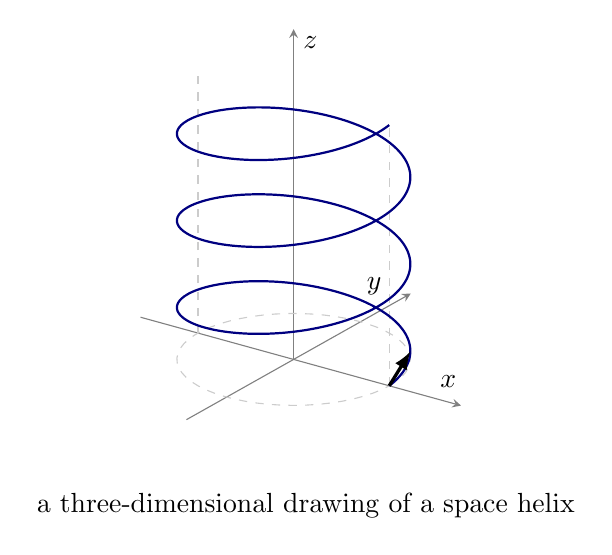
\begin{tikzpicture}[>=latex]

    \begin{axis}[
        name=helixplot,
        view={35}{25},
        width=8.5cm, height=8.5cm,
        axis lines=center,
        axis line style={gray, thin},
        xlabel={\(x\)}, ylabel={\(y\)}, zlabel={\(z\)},
        ticks=none,
        xmin=-3.2, xmax=3.5,
        ymin=-3.2, ymax=3.5,
        zmin=0, zmax=3.8,
    ]

        % Bounding cylinder base for depth perception
        \addplot3[
            gray!40, dashed, 
            domain=0:360, 
            samples=60,
            samples y=0,
            variable=\t
        ] ({2*cos(\t)}, {2*sin(\t)}, 0);
        
        % Vertical bounding lines
        \draw[gray!40, dashed] (2,0,0) -- (2,0,3);
        \draw[gray!40, dashed] (-2,0,0) -- (-2,0,3);

        % 3D Helix 
        % 3 full turns = 1080 degrees. z = t/(2pi) -> t/360.
        \addplot3[
            thick, blue!50!black,
            domain=0:1080,
            samples=250,
            samples y=0,
            variable=\t,
            smooth
        ] ({2*cos(\t)}, {2*sin(\t)}, {\t/360});

        % Displacement vector from t=0 to t=0.6 radians
        \draw[->, very thick] (2,0,0) -- ({2*cos(deg(0.6))}, {2*sin(deg(0.6))}, {0.6/(2*pi)});

    \end{axis}
    
    % Label positioned neatly below the axis environment
    \node[align=center] at ([yshift=-0.5cm]helixplot.south) {a three-dimensional drawing of a space helix};

\end{tikzpicture}
\caption{A helix can be viewed as circular motion together with steady upward motion.}
\end{figure}
\end{example}

The helix is not the graph of a single function \(y=f(x)\).  It can pass over the same
\(x\)-value many times.  Parametric equations are more flexible than ordinary graph
equations because each coordinate is allowed to depend on the parameter.

\subsection{Eliminating the parameter when possible}

Sometimes a parametric curve can be rewritten as a familiar Cartesian equation.

\begin{example}[A parabola from a moving point]
Let
\[
    \mathbf r(t)=(t,t^2),\qquad -2\le t\le2.
\]
Then
\[
    x=t,\qquad y=t^2.
\]
Since \(x=t\), we get
\[
    y=x^2.
\]
So this parametrization traces the part of the parabola \(y=x^2\) with
\[
    -2\le x\le2.
\]
\end{example}

The parameter was easy to eliminate because one coordinate was just \(t\).

\begin{example}[A circle from trigonometry]
For
\[
    \mathbf r(t)=(3\cos t,3\sin t),
\]
we have
\[
    x=3\cos t,\qquad y=3\sin t.
\]
Squaring and adding gives
\[
    x^2+y^2
    =
    9\cos^2t+9\sin^2t
    =
    9.
\]
So the image lies on
\[
    x^2+y^2=9.
\]
If \(0\le t\le2\pi\), every point on this circle is reached.
\end{example}

Eliminating the parameter can help us recognize the shape.  But it can also hide
important information.

\begin{example}[Elimination can lose information]
Consider
\[
    \mathbf r(t)=(t^2,t^4),\qquad -2\le t\le2.
\]
Then
\[
    x=t^2,\qquad y=t^4.
\]
Since
\[
    y=(t^2)^2,
\]
we get
\[
    y=x^2.
\]
But this parametrization does \emph{not} trace the whole parabola \(y=x^2\).  Because
\[
    x=t^2\ge0,
\]
it only traces the right-hand half:
\[
    y=x^2,\qquad 0\le x\le4.
\]
Also, most points are traced twice: once by \(t\) and once by \(-t\).
\end{example}

The Cartesian equation tells us the set of points.  The parametrization tells us how the
set is traveled.

\subsection{Different parametrizations of the same curve}

The same geometric curve may have many different parametrizations.

\begin{example}[Same circle, different clocks]
The two parametrizations
\[
    \mathbf r_1(t)=(\cos t,\sin t),
    \qquad 0\le t\le2\pi,
\]
and
\[
    \mathbf r_2(s)=(\cos 2s,\sin 2s),
    \qquad 0\le s\le\pi,
\]
trace the same unit circle once in the counterclockwise direction.

The second curve uses a different clock.  When \(s\) increases by \(\pi\), the angle
\(2s\) increases by \(2\pi\), so the point completes one full turn.
\end{example}

\begin{example}[Same circle, opposite direction]
The parametrization
\[
    \mathbf r_3(t)=(\cos t,-\sin t),
    \qquad 0\le t\le2\pi,
\]
also traces the unit circle.  But it moves clockwise.

At \(t=0\),
\[
    \mathbf r_3(0)=(1,0).
\]
At \(t=\pi/2\),
\[
    \mathbf r_3(\pi/2)=(0,-1).
\]
So the point goes downward first, not upward.
\end{example}

\begin{definition}[Orientation of a parametrized curve]
The direction in which a parametrized curve is traced as the parameter increases is
called its \emph{orientation}.
\end{definition}

Orientation will matter later.  If we integrate a \(1\)-form along a curve, reversing the
curve reverses the sign of the integral.  This is the one-dimensional version of the
orientation signs we saw in determinants and wedge products:
\[
    dx\wedge dy=-dy\wedge dx.
\]

\begin{definition}[Closed and simple curves]
A parametrized curve
\[
    \mathbf r:[a,b]\to\mathbb R^n
\]
is called \emph{closed} if
\[
    \mathbf r(a)=\mathbf r(b).
\]

It is called \emph{simple} if it does not pass through the same point twice, except
possibly at the endpoints of a closed curve.
\end{definition}

A circle traced once is closed and simple.  A figure-eight curve is closed but not simple,
because it crosses itself.

\begin{example}[A curve with a self-crossing]
Let
\[
    \mathbf r(t)=(\sin t,\sin 2t),
    \qquad 0\le t\le2\pi.
\]
At
\[
    t=0,\quad t=\pi,\quad t=2\pi,
\]
the point is
\[
    (0,0).
\]
The curve returns to the origin in the middle of its trip, so it has a self-crossing.
\end{example}

A curve is therefore more than its equation and more than its picture.  It is a moving
point with a chosen parameter and a chosen direction.

Rectangular coordinates describe many curves well, but they are clumsy for curves
that circle around a point.  The circle
\[
    x^2+y^2=9
\]
looks simpler as ``distance from the origin equals \(3\).''  That sentence is not written
in \(x\) and \(y\).  It is written in distance and angle.  The next coordinate system is
built for exactly that language.

\section{Polar coordinates}
\label{sec:4.2}

The circle in Section \ref{sec:4.1} kept producing the same pair of functions:
\[
    x=3\cos t,\qquad y=3\sin t.
\]
This was not an accident.  Rectangular coordinates describe a point by its shadows on
two perpendicular axes.  For a point moving around a center, another description is often
more natural:

\[
    \text{How far from the center?}
    \qquad
    \text{At what angle?}
\]

That is polar coordinates.

\subsection{The plane described by distance and angle}

A radar screen tracks a small boat.  The boat is \(5\) km from the radar station, in a
direction \(30^\circ\) counterclockwise from east.

In rectangular coordinates, the position is
\[
    \left(5\cos 30^\circ,5\sin 30^\circ\right)
    =
    \left(\frac{5\sqrt3}{2},\frac52\right).
\]
But the radar description itself is shorter:
\[
    (r,\theta)=\left(5,\frac{\pi}{6}\right).
\]
Here \(r\) is distance from the origin, and \(\theta\) is angle from the positive
\(x\)-axis.

\begin{figure}[h]
\centering
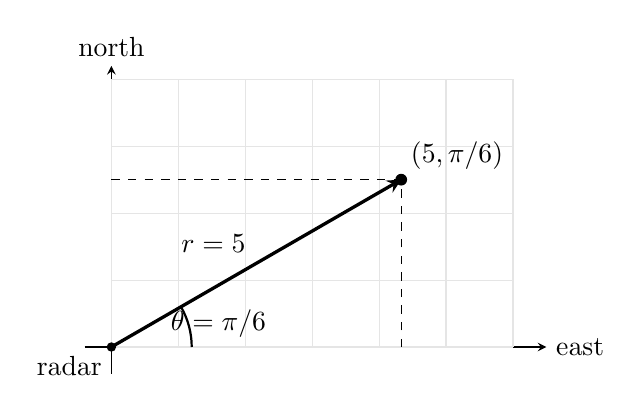
\begin{tikzpicture}[scale=0.85, >=stealth]
    \draw[->] (-0.4,0) -- (6.5,0) node[right] {east};
    \draw[->] (0,-0.4) -- (0,4.2) node[above] {north};

    \draw[gray!20, step=1] (0,0) grid (6,4);

    \draw[->, very thick] (0,0) -- ({5*cos(30)}, {5*sin(30)})
        node[midway, above left] {\(r=5\)};

    \draw[dashed] ({5*cos(30)},0) -- ({5*cos(30)}, {5*sin(30)});
    \draw[dashed] (0,{5*sin(30)}) -- ({5*cos(30)}, {5*sin(30)});

    \draw[thick] (1.2,0) arc[start angle=0,end angle=30,radius=1.2];
    \node at (1.6,0.35) {\(\theta=\pi/6\)};

    \fill ({5*cos(30)}, {5*sin(30)}) circle (2.5pt);
    \node[above right] at ({5*cos(30)}, {5*sin(30)})
        {\(\left(5,\pi/6\right)\)};

    \fill (0,0) circle (2pt);
    \node[below left] at (0,0) {radar};
\end{tikzpicture}
\caption{Polar coordinates describe a point by distance from the origin and angle from
the positive \(x\)-axis.}
\end{figure}

\begin{definition}[Polar coordinates]
The \emph{polar coordinates} of a point in the plane are written
\[
    (r,\theta).
\]
The number \(r\) is the distance from the origin, and \(\theta\) is the angle measured
counterclockwise from the positive \(x\)-axis.

The positive \(x\)-axis is called the \emph{polar axis}.
\end{definition}

The origin is called the \emph{pole}.  When \(r=0\), the angle does not matter.  All
of these describe the same point:
\[
    (0,0),\qquad
    \left(0,\frac{\pi}{3}\right),\qquad
    (0,100).
\]

\subsection{Converting between polar and Cartesian coordinates}

The conversion formulas come directly from right-triangle trigonometry:
\[
\boxed{
    x=r\cos\theta,\qquad y=r\sin\theta.
}
\]
Also,
\[
\boxed{
    r^2=x^2+y^2.
}
\]
When \(x\neq0\),
\[
    \tan\theta=\frac{y}{x},
\]
but this last formula must be used carefully because tangent does not determine the
quadrant by itself.

\begin{example}[From polar to Cartesian]
Convert
\[
    (r,\theta)=\left(4,\frac{\pi}{3}\right)
\]
to Cartesian coordinates.

Using
\[
    x=r\cos\theta,\qquad y=r\sin\theta,
\]
we get
\[
    x=4\cos\frac{\pi}{3}=4\cdot\frac12=2,
\]
and
\[
    y=4\sin\frac{\pi}{3}=4\cdot\frac{\sqrt3}{2}=2\sqrt3.
\]
So
\[
    \left(4,\frac{\pi}{3}\right)
    =
    (2,2\sqrt3)
\]
in Cartesian coordinates.
\end{example}

\begin{example}[From Cartesian to polar]
Find polar coordinates for
\[
    (-3,3).
\]
First,
\[
    r=\sqrt{(-3)^2+3^2}=\sqrt{18}=3\sqrt2.
\]
The point lies in the second quadrant.  The reference angle is \(\pi/4\), so one possible
angle is
\[
    \theta=\frac{3\pi}{4}.
\]
Thus one polar description is
\[
    \left(3\sqrt2,\frac{3\pi}{4}\right).
\]
\end{example}

The quadrant matters.  The points
\[
    (1,1)
    \qquad\text{and}\qquad
    (-1,-1)
\]
both satisfy
\[
    \frac{y}{x}=1.
\]
So both have
\[
    \tan\theta=1.
\]
But their angles are different:
\[
    (1,1) \text{ has angle } \frac{\pi}{4},
\]
while
\[
    (-1,-1) \text{ has angle } \frac{5\pi}{4}.
\]
The tangent ratio alone cannot see the quadrant.

\subsection{Polar coordinates are not unique}

Rectangular coordinates are unique: a point has exactly one pair \((x,y)\).  Polar
coordinates are different.

The angle can always be changed by a full turn:
\[
    (r,\theta)=(r,\theta+2\pi)=(r,\theta-2\pi).
\]
For example,
\[
    \left(5,\frac{\pi}{6}\right)
\]
and
\[
    \left(5,\frac{13\pi}{6}\right)
\]
represent the same point.

There is another source of non-uniqueness.  If we allow negative \(r\), then
\[
    (-r,\theta)
\]
means: go distance \(r\) in the opposite direction.  Equivalently,
\[
\boxed{
    (-r,\theta)=(r,\theta+\pi).
}
\]
For example,
\[
    \left(-2,\frac{\pi}{4}\right)
    =
    \left(2,\frac{5\pi}{4}\right).
\]

\begin{example}[Three names for one point]
The point with polar coordinates
\[
    \left(3,\frac{\pi}{3}\right)
\]
also has coordinates
\[
    \left(3,\frac{7\pi}{3}\right)
\]
because adding \(2\pi\) does not change the direction.

It also has coordinates
\[
    \left(-3,\frac{4\pi}{3}\right)
\]
because a negative radius reverses the direction by \(\pi\).
\end{example}

This non-uniqueness is not a mistake.  It is part of what makes polar equations flexible.
Some polar curves are much simpler if negative values of \(r\) are allowed.

\subsection{Polar graphs and their symmetries}

A polar equation relates \(r\) and \(\theta\).  The most common kind has the form
\[
    r=f(\theta).
\]
To graph it, choose an angle \(\theta\), compute \(r\), and plot the point
\[
    (r,\theta).
\]

\begin{example}[The equation \(r=3\)]
The polar equation
\[
    r=3
\]
means that every point is distance \(3\) from the origin.  The angle is free.  Therefore
the graph is the circle
\[
    x^2+y^2=9.
\]
\end{example}

\begin{example}[The equation \(\theta=\pi/4\)]
The polar equation
\[
    \theta=\frac{\pi}{4}
\]
means that the direction is fixed and the distance may vary.  The graph is the line
through the origin making angle \(\pi/4\) with the positive \(x\)-axis.

If we allow negative \(r\), then the same equation gives the whole line.  If we require
\(r\ge0\), it gives only one ray.
\end{example}

Symmetry can often be read from the equation before drawing the whole curve.

\[
\begin{array}{c|c}
\text{Polar behavior} & \text{Geometric symmetry} \\ \hline
r(-\theta)=r(\theta) & \text{symmetry across the }x\text{-axis}\\[2mm]
r(\pi-\theta)=r(\theta) & \text{symmetry across the }y\text{-axis}\\[2mm]
r(\theta+\pi)=r(\theta) & \text{symmetry through the origin}
\end{array}
\]

\begin{example}[A symmetric curve]
The curve
\[
    r=2+\cos\theta
\]
is symmetric across the \(x\)-axis because
\[
    r(-\theta)=2+\cos(-\theta)=2+\cos\theta=r(\theta).
\]
So once we know the upper half of the graph, the lower half is its mirror image.
\end{example}

These tests are helpful, but they are not a substitute for understanding the curve.  Polar
coordinates can describe the same point in more than one way, especially when negative
values of \(r\) occur.  Symmetry tests are guides, not laws to follow blindly.

\subsection{Circles, spirals, and roses}

Polar coordinates are especially good for curves built from distance and angle.

\begin{example}[A circle not centered at the origin]
Consider
\[
    r=4\cos\theta.
\]
Multiply both sides by \(r\):
\[
    r^2=4r\cos\theta.
\]
Using
\[
    r^2=x^2+y^2,
    \qquad
    r\cos\theta=x,
\]
we get
\[
    x^2+y^2=4x.
\]
Complete the square:
\[
    x^2-4x+y^2=0,
\]
so
\[
    (x-2)^2+y^2=4.
\]
This is a circle centered at \((2,0)\) with radius \(2\).

\begin{figure}[h]
\centering
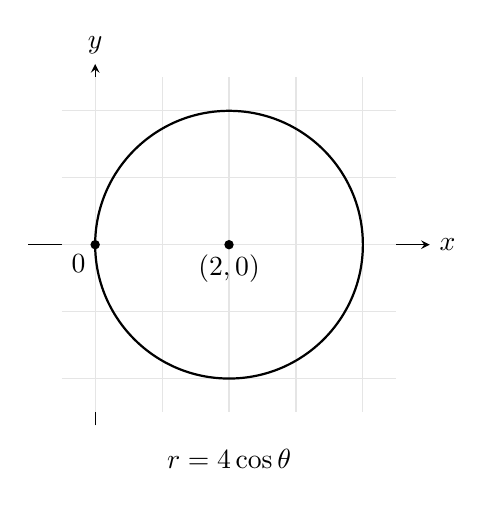
\begin{tikzpicture}[scale=0.85, >=stealth]
    \draw[->] (-1,0) -- (5,0) node[right] {\(x\)};
    \draw[->] (0,-2.7) -- (0,2.7) node[above] {\(y\)};

    \draw[gray!20, step=1] (-0.5,-2.5) grid (4.5,2.5);

    \draw[thick] (2,0) circle (2);

    \fill (2,0) circle (2pt);
    \node[below] at (2,0) {\((2,0)\)};

    \fill (0,0) circle (2pt);
    \node[below left] at (0,0) {\(0\)};

    \node at (2,-3.2) {\(r=4\cos\theta\)};
\end{tikzpicture}
\caption{The polar equation \(r=4\cos\theta\) is a circle tangent to the origin.}
\end{figure}
\end{example}

This example shows why polar equations can be surprising.  A simple expression in
\(r\) and \(\theta\) may hide a familiar Cartesian curve.

\begin{example}[An Archimedean spiral]
The polar equation
\[
    r=\frac{\theta}{4},
    \qquad 0\le\theta\le6\pi,
\]
describes a point whose distance from the origin grows steadily as the angle turns.
The result is a spiral.

\begin{figure}[h]
\centering
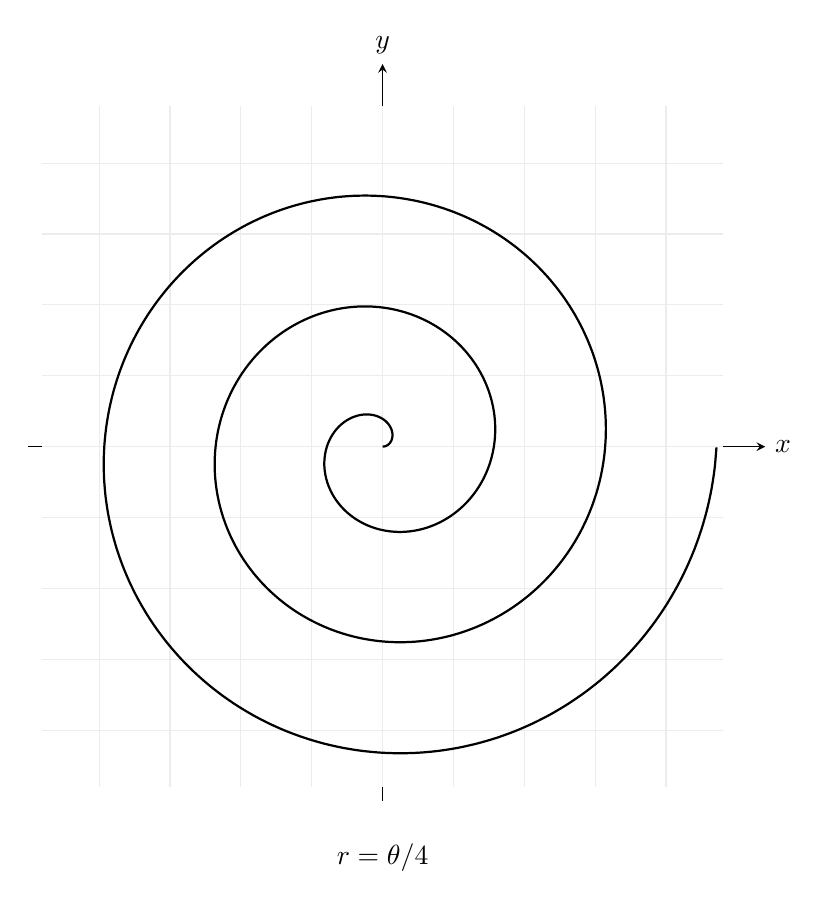
\begin{tikzpicture}[scale=0.9, >=stealth]
    \draw[->] (-5,0) -- (5.4,0) node[right] {\(x\)};
    \draw[->] (0,-5) -- (0,5.4) node[above] {\(y\)};

    \draw[gray!15, step=1] (-4.8,-4.8) grid (4.8,4.8);

    \draw[thick, domain=0:18.85, samples=300, smooth, variable=\theta]
        plot ({(\theta/4)*cos(\theta r)}, {(\theta/4)*sin(\theta r)});

    \node at (0,-5.8) {\(r=\theta/4\)};
\end{tikzpicture}
\caption{A spiral appears when the distance from the origin changes with the angle.}
\end{figure}
\end{example}

\begin{example}[A rose curve]
The polar equation
\[
    r=2\cos(3\theta)
\]
produces a three-petaled rose.

When
\[
    \cos(3\theta)>0,
\]
the radius is positive.  When
\[
    \cos(3\theta)<0,
\]
the radius is negative, so the point is plotted in the opposite direction.  This sign
change is what helps create petals.

\begin{figure}[h]
\centering
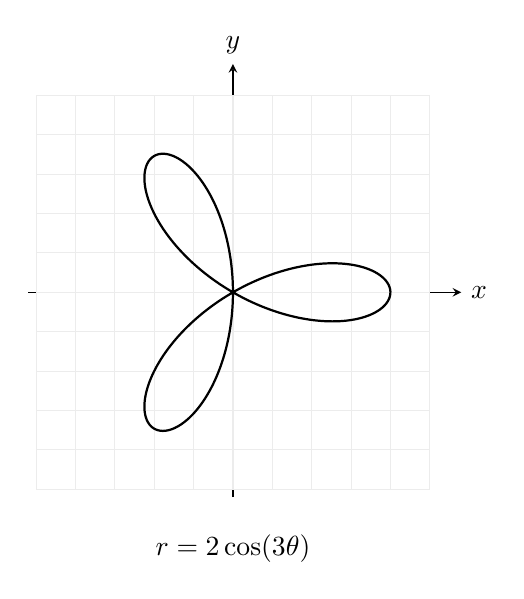
\begin{tikzpicture}[scale=1.0, >=stealth]
    \draw[->] (-2.6,0) -- (2.9,0) node[right] {\(x\)};
    \draw[->] (0,-2.6) -- (0,2.9) node[above] {\(y\)};

    \draw[gray!15, step=0.5] (-2.5,-2.5) grid (2.5,2.5);

    \draw[thick, domain=0:6.283, samples=400, smooth, variable=\theta]
        plot ({(2*cos(3*\theta r))*cos(\theta r)},
              {(2*cos(3*\theta r))*sin(\theta r)});

    \node at (0,-3.25) {\(r=2\cos(3\theta)\)};
\end{tikzpicture}
\caption{A rose curve uses negative radius values as part of the drawing.}
\end{figure}
\end{example}

Polar coordinates are not only a way to draw pretty curves.  They are a coordinate
change:
\[
    (r,\theta)\longmapsto (r\cos\theta,r\sin\theta).
\]
This map bends a rectangular grid in the \((r,\theta)\)-plane into circles and rays in
the \((x,y)\)-plane.

\begin{figure}[h]
\centering
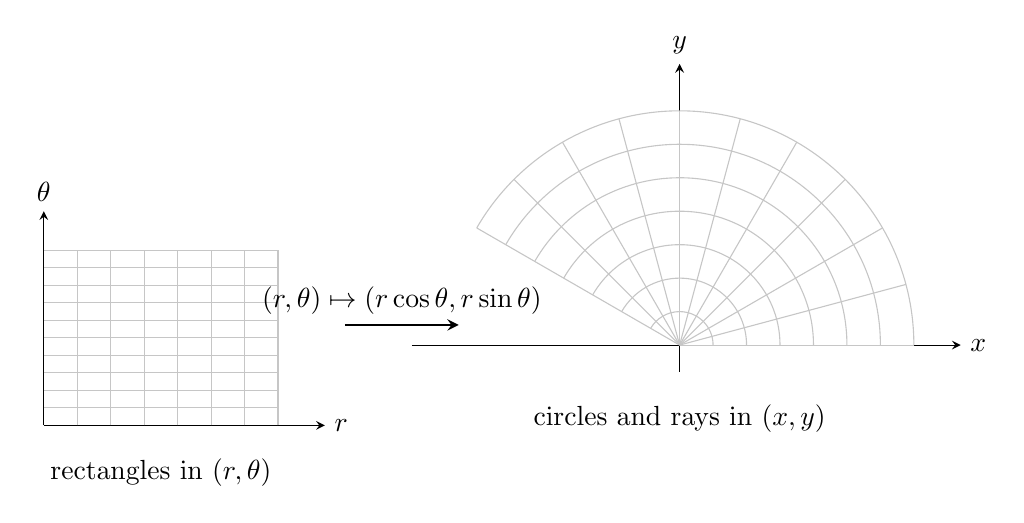
\begin{tikzpicture}[scale=0.85, >=stealth]
    \begin{scope}
        % Left grid axes
        \draw[->] (0,0) -- (4.2,0) node[right] {\(r\)};
        \draw[->] (0,0) -- (0,3.2) node[above] {\(\theta\)};

        % Vertical lines (constant r) every 0.5 up to 3.5
        \foreach \r in {0.5, 1.0, 1.5, 2.0, 2.5, 3.0, 3.5}
            \draw[gray!45] (\r,0) -- (\r,{150*pi/180});

        % Horizontal lines (constant theta) every 15 degrees exactly in radians
        \foreach \ang in {15, 30, 45, 60, 75, 90, 105, 120, 135, 150}
            \draw[gray!45] (0,{\ang*pi/180}) -- (3.5,{\ang*pi/180});

        \node at (1.75,-0.7) {rectangles in \((r,\theta)\)};
    \end{scope}

    % Shifted further right to prevent overlap
    \begin{scope}[shift={(9.5,1.2)}]
        % Right grid axes
        \draw[->] (-4.0,0) -- (4.2,0) node[right] {\(x\)};
        \draw[->] (0,-0.4) -- (0,4.2) node[above] {\(y\)};

        % Arcs (constant r) properly centered at origin by starting at (\r, 0)
        \foreach \r in {0.5, 1.0, 1.5, 2.0, 2.5, 3.0, 3.5}
            \draw[gray!45] (\r,0) arc[start angle=0, end angle=150, radius=\r];

        % Rays (constant theta) every 15 degrees, capped at outer radius 3.5
        \foreach \ang in {0, 15, 30, 45, 60, 75, 90, 105, 120, 135, 150}
            \draw[gray!45] (0,0) -- (\ang:3.5);

        \node at (0,-1.1) {circles and rays in \((x,y)\)};
    \end{scope}

    % Mapping arrow
    \draw[->, thick] (4.5, 1.5) -- (6.2, 1.5)
        node[midway, above] {\((r,\theta)\mapsto(r\cos\theta,r\sin\theta)\)};
\end{tikzpicture}
\caption{The polar coordinate map turns a rectangular coordinate grid into a curved grid.}
\end{figure}

This curved grid carries a hidden warning.  A small change \(\Delta\theta\) sweeps a
short arc near the origin but a longer arc farther away.  So a tiny polar rectangle with
side lengths \(\Delta r\) and \(\Delta\theta\) does not have area
\[
    \Delta r\,\Delta\theta.
\]
The angular side has length about
\[
    r\,\Delta\theta.
\]
That factor \(r\) will return later in integrals as
\[
    r\,dr\,d\theta,
\]
and in the language of forms as the coefficient in
\[
    dx\wedge dy
    =
    r\,dr\wedge d\theta.
\]

Polar coordinates solve circular problems in the plane.  But a pipe has height, a sphere
has latitude as well as longitude, and a planet is better described by distance and two
angles than by \(x,y,z\).  The next step is to let polar coordinates grow upward into
space: first into cylindrical coordinates, then into spherical coordinates.
\section{Cylindrical and spherical coordinates}
\label{sec:4.3}

Polar coordinates gave us a better language for circular motion in the plane:
\[
    (r,\theta)\longmapsto (r\cos\theta,r\sin\theta).
\]
At the end of Section \ref{sec:4.2}, we saw that this coordinate map bends a rectangular
\((r,\theta)\)-grid into circles and rays.  It also brought a warning: angular motion has
different physical length depending on how far we are from the origin.

Now we lift that idea into space.

A point in space can be described by its rectangular coordinates
\[
    (x,y,z).
\]
But if the object is a pipe, a silo, a planet, a cone of light, or a sphere, rectangular
coordinates often hide the shape.  Circular and spherical objects ask for circular and
spherical coordinates.

\subsection{Cylindrical coordinates as polar coordinates with height}

Imagine a worker standing inside a round grain silo.  To describe her location, it is
natural to say:

\[
    \text{distance from the center axis},\qquad
    \text{angle around the silo},\qquad
    \text{height above the floor}.
\]

That is not a new idea.  It is just polar coordinates in the floor, together with the old
vertical coordinate \(z\).

\begin{example}[A point in a round silo]
Suppose a point is
\[
    4 \text{ meters from the center axis},
\]
at angle
\[
    \theta=\frac{\pi}{6},
\]
and at height
\[
    z=7.
\]
Then its cylindrical coordinates are
\[
    \left(4,\frac{\pi}{6},7\right).
\]
To convert to rectangular coordinates, use the polar formulas in the \(xy\)-plane:
\[
    x=r\cos\theta,\qquad y=r\sin\theta.
\]
So
\[
    x=4\cos\frac{\pi}{6}=4\cdot\frac{\sqrt3}{2}=2\sqrt3,
\]
and
\[
    y=4\sin\frac{\pi}{6}=4\cdot\frac12=2.
\]
The height remains
\[
    z=7.
\]
Thus
\[
    \left(4,\frac{\pi}{6},7\right)
    =
    (2\sqrt3,2,7)
\]
in rectangular coordinates.
\end{example}

\begin{definition}[Cylindrical coordinates]
The \emph{cylindrical coordinates} of a point in space are written
\[
    (r,\theta,z).
\]
The first two coordinates \((r,\theta)\) are polar coordinates in the \(xy\)-plane, and
\(z\) is the usual height coordinate.

The conversion formulas are
\[
\boxed{
    x=r\cos\theta,\qquad y=r\sin\theta,\qquad z=z.
}
\]
Also,
\[
\boxed{
    r^2=x^2+y^2.
}
\]
\end{definition}

The repeated symbol \(z=z\) in the conversion formula is not a joke.  It says that the
height coordinate is unchanged.  Cylindrical coordinates change how we describe motion
around the vertical axis, but they keep the vertical direction as it was.

\begin{figure}[h]
\centering
\begin{tikzpicture}[scale=0.85, >=stealth]
    % axes
    \draw[->] (0,0) -- (5.2,0) node[right] {\(x\)};
    \draw[->] (0,0) -- (-2.2,-1.5) node[left] {\(y\)};
    \draw[->] (0,0) -- (0,5.1) node[above] {\(z\)};

    % floor ellipse
    \draw[gray!50] (0,0) ellipse (2.4 and 0.8);

    % point projection
    \coordinate (O) at (0,0);
    \coordinate (Pxy) at (2.0,-0.55);
    \coordinate (P) at (2.0,3.4);

    \draw[dashed] (Pxy) -- (P);
    \draw[->, thick] (O) -- (Pxy) node[midway, below] {\(r\)};
    \draw[->, thick] (Pxy) -- (P) node[midway, right] {\(z\)};

    \draw[thick] (0.9,0) arc[start angle=0,end angle=-15,x radius=1.0,y radius=0.35];
    \node at (1.25,-0.28) {\(\theta\)};

    \fill (P) circle (2.5pt);
    \fill (Pxy) circle (2pt);
    \node[right] at (P) {\((r,\theta,z)\)};

    \draw[dashed] (0,3.4) -- (P);
\end{tikzpicture}
\caption{Cylindrical coordinates use polar coordinates in the horizontal plane and keep
the usual height coordinate.}
\end{figure}

\begin{example}[From rectangular to cylindrical]
Find cylindrical coordinates for
\[
    (x,y,z)=(-3,3,5).
\]
First,
\[
    r=\sqrt{x^2+y^2}=\sqrt{(-3)^2+3^2}=3\sqrt2.
\]
The point \((-3,3)\) lies in the second quadrant of the \(xy\)-plane, so one possible
angle is
\[
    \theta=\frac{3\pi}{4}.
\]
The height is unchanged:
\[
    z=5.
\]
Thus one cylindrical description is
\[
    \left(3\sqrt2,\frac{3\pi}{4},5\right).
\]
\end{example}

Cylindrical coordinates are not unique, because the angle is not unique:
\[
    (r,\theta,z)=(r,\theta+2\pi,z).
\]
Also, if \(r=0\), the angle does not matter.  Every point on the \(z\)-axis has the form
\[
    (0,\theta,z),
\]
for any angle \(\theta\).

Usually we take
\[
    r\ge0.
\]
Negative radii can be allowed, just as in polar coordinates, but most multivariable
calculus problems avoid them in cylindrical coordinates because the standard range
\(r\ge0\) already describes space cleanly.

\subsection{Coordinate surfaces in cylindrical coordinates}

A coordinate system gives us a grid.  In three dimensions, the grid is made from
surfaces, not lines.

In cylindrical coordinates, each coordinate surface comes from holding one coordinate
constant.

\[
\begin{array}{c|c}
\text{Fixed coordinate} & \text{Surface in space} \\ \hline
r=a & \text{circular cylinder of radius }a\\[1mm]
\theta=\alpha & \text{vertical half-plane through the }z\text{-axis}\\[1mm]
z=c & \text{horizontal plane}
\end{array}
\]

\begin{example}[A pipe as a coordinate surface]
The equation
\[
    r=3
\]
means every point is distance \(3\) from the \(z\)-axis.  In rectangular coordinates,
this is
\[
    x^2+y^2=9.
\]
There is no restriction on \(z\), so the graph is an infinite circular cylinder.
\end{example}

\begin{example}[A cone in cylindrical coordinates]
The equation
\[
    z=r
\]
says that the height equals the distance from the \(z\)-axis.  In rectangular coordinates,
\[
    z=\sqrt{x^2+y^2}.
\]
Squaring gives
\[
    z^2=x^2+y^2,
\]
with the extra condition
\[
    z\ge0.
\]
So this is the upper half of a circular cone.
\end{example}

The equation \(z=r\) is much easier to read in cylindrical coordinates than in rectangular
coordinates.  It says: as you move one unit away from the central axis, you rise one unit.

\begin{figure}[h]
\centering
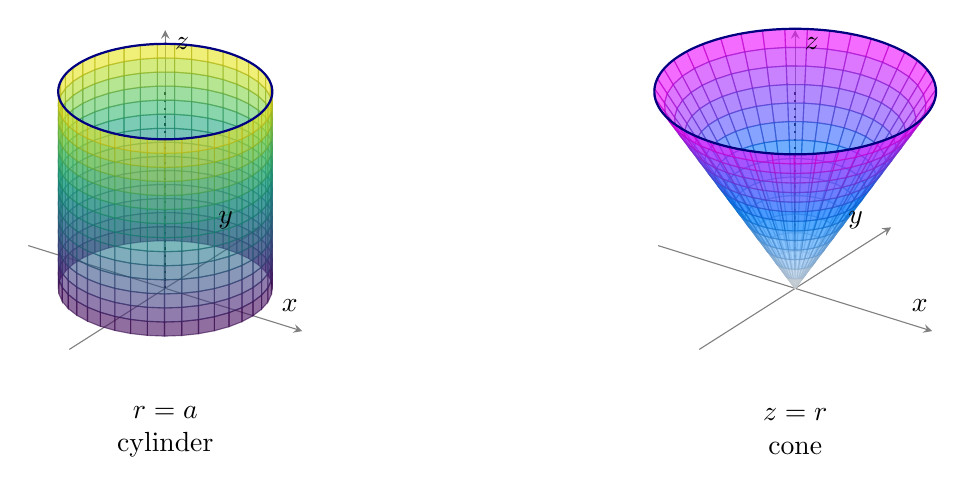
\begin{tikzpicture}[>=latex]

    % --- CYLINDER ---
    \begin{axis}[
        name=cylinderplot,
        view={35}{30},
        width=7.5cm, height=7.5cm,
        axis lines=center,
        axis line style={gray, thin},
        xlabel={\(x\)}, ylabel={\(y\)}, zlabel={\(z\)},
        ticks=none,
        xmin=-2.5, xmax=2.5,
        ymin=-2.5, ymax=2.5,
        zmin=0, zmax=4.2,
        ]
        
        % Dotted internal vertical axis
        \addplot3[dotted, thick] coordinates {(0,0,0) (0,0,3.2)};

        % Main surface
        \addplot3[
            surf,
            colormap/viridis,
            opacity=0.6,
            samples=40,
            samples y=15,
            domain=0:360,
            domain y=0:3.2,
            z buffer=sort
        ] ({1.6*cos(x)}, {1.6*sin(x)}, {y});

        % Top rim edge
        \addplot3[
            smooth,
            blue!50!black, thick,
            domain=0:360,
            samples=60
        ] ({1.6*cos(x)}, {1.6*sin(x)}, {3.2});
        
    \end{axis}
    
    % Labels below cylinder
    \node[align=center] at ([yshift=-0.5cm]cylinderplot.south) {\(r=a\)\\cylinder};

    % --- CONE ---
    \begin{axis}[
        name=coneplot,
        at={(8cm,0)}, % Shifted right
        view={35}{30},
        width=7.5cm, height=7.5cm,
        axis lines=center,
        axis line style={gray, thin},
        xlabel={\(x\)}, ylabel={\(y\)}, zlabel={\(z\)},
        ticks=none,
        xmin=-3.8, xmax=3.8,
        ymin=-3.8, ymax=3.8,
        zmin=0, zmax=4.2,
        ]
        
        % Dotted internal vertical axis
        \addplot3[dotted, thick] coordinates {(0,0,0) (0,0,3.2)};

        % Main surface (z=r parameterization)
        % x maps to theta, y maps to r and z
        \addplot3[
            surf,
            colormap/cool,
            opacity=0.6,
            samples=40,
            samples y=15,
            domain=0:360,
            domain y=0:3.2,
            z buffer=sort
        ] ({y*cos(x)}, {y*sin(x)}, {y});

        % Top rim edge
        \addplot3[
            smooth,
            blue!50!black, thick,
            domain=0:360,
            samples=60
        ] ({3.2*cos(x)}, {3.2*sin(x)}, {3.2});
        
    \end{axis}
    
    % Labels below cone
    \node[align=center] at ([yshift=-0.5cm]coneplot.south) {\(z=r\)\\cone};

\end{tikzpicture}
\caption{Cylindrical coordinates make cylinders and cones simple to describe.}
\end{figure}

\subsection{Spherical coordinates as radius and two angles}

Cylindrical coordinates are built around an axis.  Spherical coordinates are built around
a point.

Imagine a small drone flying near a weather balloon.  The balloon is the origin.  To
describe the drone's position, one natural report is:

\[
    \text{how far from the balloon},
\]
\[
    \text{which compass direction around the vertical axis},
\]
\[
    \text{how far down from the positive vertical axis}.
\]

That is spherical coordinates.

\begin{example}[A point described by distance and two angles]
A point is
\[
    \rho=6
\]
units from the origin.  Its horizontal direction is
\[
    \theta=\frac{\pi}{3},
\]
and its angle down from the positive \(z\)-axis is
\[
    \phi=\frac{\pi}{4}.
\]
The point has spherical coordinates
\[
    \left(6,\frac{\pi}{3},\frac{\pi}{4}\right),
\]
where the coordinates are listed as
\[
    (\rho,\theta,\phi).
\]

Its rectangular coordinates are
\[
    x=\rho\sin\phi\cos\theta,
    \qquad
    y=\rho\sin\phi\sin\theta,
    \qquad
    z=\rho\cos\phi.
\]
Therefore
\[
    x=6\sin\frac{\pi}{4}\cos\frac{\pi}{3}
    =
    6\cdot\frac{\sqrt2}{2}\cdot\frac12
    =
    \frac{3\sqrt2}{2},
\]
\[
    y=6\sin\frac{\pi}{4}\sin\frac{\pi}{3}
    =
    6\cdot\frac{\sqrt2}{2}\cdot\frac{\sqrt3}{2}
    =
    \frac{3\sqrt6}{2},
\]
and
\[
    z=6\cos\frac{\pi}{4}
    =
    3\sqrt2.
\]
\end{example}

\begin{definition}[Spherical coordinates]
The \emph{spherical coordinates} of a point in space are written
\[
    (\rho,\theta,\phi).
\]
Here

\[
\begin{array}{c|c}
\rho & \text{distance from the origin}\\
\theta & \text{angle around the }z\text{-axis, measured in the }xy\text{-plane}\\
\phi & \text{angle down from the positive }z\text{-axis}
\end{array}
\]

The conversion formulas are
\[
\boxed{
    x=\rho\sin\phi\cos\theta,\qquad
    y=\rho\sin\phi\sin\theta,\qquad
    z=\rho\cos\phi.
}
\]
\end{definition}

The angle \(\theta\) is the same angle used in polar and cylindrical coordinates.  The new
angle is \(\phi\), which measures how far the point has tilted away from the positive
\(z\)-axis.

A useful way to remember the formulas is this:

First project the point down to the \(xy\)-plane.  The projected radius is
\[
    r=\rho\sin\phi.
\]
Then use polar coordinates in that plane:
\[
    x=r\cos\theta,
    \qquad
    y=r\sin\theta.
\]
So
\[
    x=\rho\sin\phi\cos\theta,
    \qquad
    y=\rho\sin\phi\sin\theta.
\]
The vertical coordinate is
\[
    z=\rho\cos\phi.
\]

\begin{figure}[h]
\centering
\begin{tikzpicture}[scale=0.9, >=stealth]
    \draw[->] (0,0) -- (4.8,0) node[right] {\(x\)};
    \draw[->] (0,0) -- (-1.9,-1.2) node[left] {\(y\)};
    \draw[->] (0,0) -- (0,4.6) node[above] {\(z\)};

    \coordinate (O) at (0,0);
    \coordinate (Pxy) at (2.7,-0.7);
    \coordinate (P) at (2.7,3.0);

    \draw[dashed] (Pxy) -- (P);
    \draw[dashed] (O) -- (Pxy);
    \draw[->, very thick] (O) -- (P) node[midway, above left] {\(\rho\)};

    \draw[thick] (0,1.2) arc[start angle=90,end angle=48,radius=1.2];
    \node at (0.7,1.55) {\(\phi\)};

    \draw[thick] (0.9,0) arc[start angle=0,end angle=-14,x radius=1.0,y radius=0.32];
    \node at (1.35,-0.27) {\(\theta\)};

    \draw[->, thick] (O) -- (Pxy) node[midway, below] {\(\rho\sin\phi\)};
    \fill (P) circle (2.5pt);
    \fill (Pxy) circle (2pt);
    \node[right] at (P) {\((\rho,\theta,\phi)\)};
\end{tikzpicture}
\caption{Spherical coordinates use one distance \(\rho\) and two angles \(\theta\) and
\(\phi\).}
\end{figure}

\begin{example}[From rectangular to spherical]
Find spherical coordinates for
\[
    (x,y,z)=(1,1,\sqrt2).
\]
First,
\[
    \rho=\sqrt{x^2+y^2+z^2}
    =
    \sqrt{1^2+1^2+(\sqrt2)^2}
    =
    \sqrt4
    =
    2.
\]
The angle around the \(z\)-axis is found from the projection \((1,1)\) in the
\(xy\)-plane:
\[
    \theta=\frac{\pi}{4}.
\]
Finally,
\[
    z=\rho\cos\phi.
\]
So
\[
    \sqrt2=2\cos\phi,
\]
which gives
\[
    \cos\phi=\frac{\sqrt2}{2}.
\]
Thus
\[
    \phi=\frac{\pi}{4}.
\]
One spherical description is
\[
    \left(2,\frac{\pi}{4},\frac{\pi}{4}\right).
\]
\end{example}

For converting from rectangular to spherical, the main formulas are
\[
\boxed{
    \rho^2=x^2+y^2+z^2,
}
\]
\[
\boxed{
    \tan\theta=\frac{y}{x}
    \quad\text{with the quadrant checked carefully},
}
\]
and
\[
\boxed{
    \cos\phi=\frac{z}{\rho}
    \quad(\rho\neq0).
}
\]

As always, angle formulas need care.  The equation
\[
    \tan\theta=\frac{y}{x}
\]
does not determine the quadrant by itself.

\subsection{Coordinate surfaces in spherical coordinates}

Spherical coordinates have their own grid surfaces.

\[
\begin{array}{c|c}
\text{Fixed coordinate} & \text{Surface in space} \\ \hline
\rho=a & \text{sphere of radius }a\\[1mm]
\theta=\alpha & \text{vertical half-plane through the }z\text{-axis}\\[1mm]
\phi=\beta & \text{cone with vertex at the origin}
\end{array}
\]

\begin{example}[A sphere]
The equation
\[
    \rho=5
\]
means the distance from the origin is \(5\).  In rectangular coordinates,
\[
    x^2+y^2+z^2=25.
\]
So \(\rho=5\) is the sphere of radius \(5\) centered at the origin.
\end{example}

\begin{example}[A cone]
The equation
\[
    \phi=\frac{\pi}{4}
\]
means every point makes a \(45^\circ\) angle with the positive \(z\)-axis.  Since
\[
    r=\rho\sin\phi
    \qquad\text{and}\qquad
    z=\rho\cos\phi,
\]
when \(\phi=\pi/4\) we have
\[
    r=z.
\]
So
\[
    z=\sqrt{x^2+y^2}.
\]
This is the upper cone
\[
    z^2=x^2+y^2,
    \qquad z\ge0.
\]
\end{example}

Spherical coordinates are not unique.  We can always add \(2\pi\) to \(\theta\):
\[
    (\rho,\theta,\phi)
    =
    (\rho,\theta+2\pi,\phi).
\]
At the origin, \(\rho=0\), both angles are irrelevant.  At the north and south poles,
where
\[
    \phi=0
    \quad\text{or}\quad
    \phi=\pi,
\]
the angle \(\theta\) is irrelevant because all horizontal directions meet at the same
point.

There is also a convention warning.  Some books use the letters \(\theta\) and \(\phi\)
in the opposite way.  In this book,
\[
    \theta \text{ goes around the } z\text{-axis},
\]
and
\[
    \phi \text{ comes down from the positive } z\text{-axis}.
\]

\subsection{When cylindrical or spherical coordinates are the natural choice}

A coordinate system is a language.  The best language is the one in which the geometry
speaks simply.

\[
\begin{array}{c|c}
\text{Geometry} & \text{Usually good coordinates} \\ \hline
\text{boxes, planes, rectangular rooms} & \text{rectangular}\\
\text{pipes, cylinders, vertical axes, spinning objects} & \text{cylindrical}\\
\text{spheres, balls, shells, distance from one center} & \text{spherical}
\end{array}
\]

\begin{example}[A thick pipe]
A pipe of inner radius \(2\), outer radius \(3\), and height \(5\) around the \(z\)-axis is
described simply by
\[
    2\le r\le3,
    \qquad
    0\le\theta\le2\pi,
    \qquad
    0\le z\le5.
\]
In rectangular coordinates, the same solid would require
\[
    4\le x^2+y^2\le9,
    \qquad
    0\le z\le5.
\]
The rectangular description is not wrong, but it hides the circular structure.
\end{example}

\begin{example}[A spherical shell]
A shell between two spheres centered at the origin, with radii \(1\) and \(4\), is described
by
\[
    1\le \rho\le4,
    \qquad
    0\le\phi\le\pi,
    \qquad
    0\le\theta\le2\pi.
\]
In rectangular coordinates, the condition becomes
\[
    1\le x^2+y^2+z^2\le16,
\]
which is readable, but the angular structure is hidden.
\end{example}

Not every problem with a circle needs cylindrical coordinates, and not every problem in
space needs spherical coordinates.  A rectangular box is easier in \(x,y,z\).  A plane
like
\[
    2x-y+z=5
\]
is usually easier in rectangular coordinates.  The goal is not to use the fanciest system.
The goal is to choose the coordinates that match the shape.

\subsection{The hidden size of coordinate boxes}

In rectangular coordinates, a tiny box with side lengths
\[
    \Delta x,\quad \Delta y,\quad \Delta z
\]
has volume approximately
\[
    \Delta x\,\Delta y\,\Delta z.
\]

Curved coordinates are different.

In cylindrical coordinates, a tiny coordinate box has side lengths approximately
\[
    \Delta r,\qquad r\,\Delta\theta,\qquad \Delta z.
\]
So its volume is approximately
\[
    r\,\Delta r\,\Delta\theta\,\Delta z.
\]
This is why cylindrical integrals later contain
\[
    r\,dr\,d\theta\,dz.
\]

In spherical coordinates, a tiny coordinate box has side lengths approximately
\[
    \Delta\rho,
    \qquad
    \rho\,\Delta\phi,
    \qquad
    \rho\sin\phi\,\Delta\theta.
\]
So its volume is approximately
\[
    \rho^2\sin\phi\,\Delta\rho\,\Delta\phi\,\Delta\theta.
\]
This is why spherical integrals later contain
\[
    \rho^2\sin\phi\,d\rho\,d\phi\,d\theta.
\]

In the language of forms, these volume factors are not decorations.  They record how
the coordinate map changes signed volume:
\[
\boxed{
    dx\wedge dy\wedge dz
    =
    r\,dr\wedge d\theta\wedge dz
}
\]
for cylindrical coordinates, and, with the positive spherical order
\((\rho,\phi,\theta)\),
\[
\boxed{
    dx\wedge dy\wedge dz
    =
    \rho^2\sin\phi\,d\rho\wedge d\phi\wedge d\theta.
}
\]
The factors
\[
    r
    \qquad\text{and}\qquad
    \rho^2\sin\phi
\]
are the three-dimensional relatives of the polar area factor \(r\).

Coordinates help us describe space.  They also help us recognize surfaces: cylinders,
cones, spheres, and shells appeared almost automatically.  But many surfaces are not
coordinate surfaces in a single coordinate system.  Some are bowls, some are saddles,
some are stretched spheres, and some are stranger than their equations first suggest.
To read them, we need one more geometric skill: slicing a surface and studying its
cross-sections.

\section{Quadric surfaces and level surfaces}
\label{sec:4.4}

A sphere can be written in spherical coordinates as
\[
    \rho=3.
\]
The same sphere can be written in rectangular coordinates as
\[
    x^2+y^2+z^2=9.
\]
One surface, two languages.

The next surfaces are the three-dimensional relatives of conic sections.  In the plane,
second-degree equations gave circles, ellipses, parabolas, and hyperbolas.  In space,
second-degree equations give cylinders, cones, paraboloids, ellipsoids, hyperboloids,
and saddles.

The trick is not to memorize a gallery.  The trick is to slice.

\subsection{A first surface from an equation}

Start with the equation
\[
    x^2+y^2=4.
\]
In the plane, this is a circle of radius \(2\).  But in space, the equation does not mention
\(z\).  That means \(z\) is free.

If
\[
    (x,y)
\]
lies on the circle, then every point
\[
    (x,y,z)
\]
lies on the surface, no matter how high or low \(z\) is.  The circle is lifted upward and
downward forever.

So
\[
    x^2+y^2=4
\]
is a circular cylinder in space.

\begin{example}[A missing variable creates a cylinder]
The equation
\[
    y=x^2
\]
is a parabola in the \(xy\)-plane.  In space, if the equation is still
\[
    y=x^2,
\]
then \(z\) is free.  Every point on the parabola can move up and down parallel to the
\(z\)-axis.

The result is a parabolic cylinder.
\end{example}

A cylinder does not have to be circular.  In multivariable calculus, a \emph{cylinder}
means a surface made by dragging a plane curve along a straight direction.

\begin{figure}[h]
\centering
\begin{tikzpicture}[>=latex]

    % --- LEFT COLUMN: CIRCULAR ---

    % Text at very top
    \node[anchor=north, font=\Large] (eq1) at (-4, 4) {\(x^2 + y^2 = 1\)};

    % 2D Circle Graph
    \draw[->] (-6, 0) -- (-2, 0) node[right] {\(x\)};
    \draw[->] (-4, -2) -- (-4, 2) node[above] {\(y\)};
    \node[below left] at (-4, 0) {0};
    \draw[thick, blue] (-4, 0) circle (1.5cm);
    \node[anchor=west] (label2d1) at (-3.2, 1.3) {2D \(\rightarrow\) Circle};
    \draw[->] (-4.6, 1.4) -- (label2d1);

    % 3D Cylinder Graph
    \begin{axis}[
        name=plot1,
        standard 3d,
        at={(-6.5cm, -9cm)}, % Shifted down 3cm
        xlabel={\(x\)}, ylabel={\(y\)}, zlabel={\(z\)},
        ]
        % Base circle on xy plane
        \addplot3[
            smooth,
            thin, dashed,
            domain=0:2*pi,
            samples=30,
            samples y=1,
            ] ({cos(deg(x))}, {sin(deg(x))}, {0});

        % Main surface (uses parameters and viridis map)
        \addplot3[
            surf,
            samples=30,
            samples y=2,
            domain=0:2*pi,
            domain y=0:2,
            z buffer=sort,
            opacity=0.6,
            colormap/viridis
        ] ({cos(deg(x))}, {sin(deg(x))}, {y});

        % Dotted axis inside
        \draw[dotted, thick] (0,0,0) -- (0,0,2.2);
        % Top rim edge (hidden lines removal is automatic in surf)
        \addplot3[
            smooth,
            blue, thick,
            domain=0:2*pi,
            samples=30,
            samples y=1,
            ] ({cos(deg(x))}, {sin(deg(x))}, {2});
    \end{axis}
    \node at (-3.3,-7.5) {0}; % Shifted down 3cm

    % Bottom label and arrow
    \node[anchor=north, font=\large] (label3d1) at (-4, -9.5) {3D \(\rightarrow\) Cylinder}; % Shifted down 3cm
    \draw[thick, ->] (label2d1.south) -- ++(0,-10.3); % Arrow lengthened by 3cm


    % --- RIGHT COLUMN: PARABOLIC ---

    % Text at very top
    \node[anchor=north, font=\Large] (eq2) at (4, 4) {\(y = x^2\)};

    % 2D Parabola Graph
    \draw[->] (2, 0) -- (6, 0) node[right] {\(x\)};
    \draw[->] (4, -1) -- (4, 3) node[above] {\(y\)};
    \node[below right] at (4, 0) {0};
    \draw[thick, blue, samples=30, domain=2.6:5.4] plot (\x, {(\x-4)^2});
    \node[anchor=west] (label2d2) at (3.5, 2.3) {2D \(\rightarrow\) Parabola};
    \draw[->] (3.0, 1.4) -- (label2d2);

    % 3D Parabolic Cylinder Graph
    \begin{axis}[
        name=plot2,
        standard 3d,
        at={(1.5cm, -9cm)}, % Shifted down 3cm
        % adjust limits for this plot shape
        ymin=0, ymax=2,
        xmin=-1.5, xmax=1.5,
        xlabel={\(x\)}, ylabel={\(y\)}, zlabel={\(z\)},
        ]
        % Main folded surface
        \addplot3[
            surf,
            samples=30,
            samples y=2,
            domain=-1.25:1.25,
            domain y=0:2,
            z buffer=sort,
            opacity=0.6,
            colormap/cool
        ] (x, {x^2}, {y});

        % Base curve
        \addplot3[
            smooth,
            thin, dashed,
            domain=-1.25:1.25,
            samples=30,
            samples y=1,
            ] (x, {x^2}, {0});

        % Dotted internal dashed lines (manually drawn vertical lines)
        \draw[dotted, thick] (0,0,0) -- (0,0,2);
        \draw[dotted, thick] (0.8,0.64,0) -- (0.8,0.64,2);
        \draw[dotted, thick] (-0.8,0.64,0) -- (-0.8,0.64,2);

        % Top rim edge
        \addplot3[
            smooth,
            blue, thick,
            domain=-1.25:1.25,
            samples=30,
            samples y=1,
            ] (x, {x^2}, {2});
    \end{axis}
    \node at (4.7,-7.5) {0}; % Shifted down 3cm

    % Bottom label and arrow
    \node[anchor=north, font=\large] (label3d2) at (4, -9.5) {3D \(\rightarrow\) Cylinder}; % Shifted down 3cm
    % Long arrow from Parabola 2D label to Cylinder 3D label
    \draw[thick, ->] (label2d2.south) -- ++(0,-11.3); % Arrow lengthened by 3cm

\end{tikzpicture}
\caption{If an equation in space is missing one variable, a plane curve is dragged along that missing direction.}
\end{figure}
\subsection{Cylinders, cones, paraboloids, and ellipsoids}

A \emph{quadric surface} is a surface in space described by a second-degree equation
in \(x,y,z\).  The simplest examples use squares and no mixed terms.

\begin{definition}[Quadric surface]
A \emph{quadric surface} is the graph or level set of a second-degree equation in
\(x,y,z\).  Typical terms include
\[
    x^2,\qquad y^2,\qquad z^2,\qquad xy,\qquad xz,\qquad yz,
\]
together with possible linear and constant terms.
\end{definition}

The word ``surface'' is a little generous.  Some second-degree equations degenerate.

For example,
\[
    x^2+y^2+z^2=-1
\]
has no real points at all.  The equation
\[
    x^2+y^2+z^2=0
\]
has only one point, the origin.  And
\[
    x^2-y^2=0
\]
factors as
\[
    (x-y)(x+y)=0,
\]
so it gives two planes:
\[
    x=y
    \qquad\text{and}\qquad
    x=-y.
\]
These warning examples remind us that equations must be read, not merely classified.

Now let us look at the main shapes.

\begin{example}[An elliptic paraboloid: a bowl]
Consider
\[
    z=\frac{x^2}{4}+y^2.
\]
At \(z=0\), the only point is
\[
    (0,0,0).
\]
At \(z=1\), we get
\[
    \frac{x^2}{4}+y^2=1,
\]
an ellipse.  At \(z=4\), we get
\[
    \frac{x^2}{4}+y^2=4,
\]
a larger ellipse.

So horizontal slices are ellipses that grow as \(z\) increases.  The surface is a bowl
opening upward.  It is called an \emph{elliptic paraboloid}.
\end{example}

The circular paraboloid
\[
    z=x^2+y^2
\]
is the special case where the horizontal slices are circles.  But most bowls are not
perfectly round; their slices may be ellipses.

\begin{example}[An ellipsoid: a stretched sphere]
The equation
\[
    \frac{x^2}{9}+\frac{y^2}{4}+z^2=1
\]
describes a stretched sphere, called an \emph{ellipsoid}.

To see the stretches, set two variables to zero.

If
\[
    y=0,\qquad z=0,
\]
then
\[
    \frac{x^2}{9}=1,
\]
so
\[
    x=\pm3.
\]
Along the \(x\)-axis, the ellipsoid reaches \(3\) units.

If
\[
    x=0,\qquad z=0,
\]
then
\[
    \frac{y^2}{4}=1,
\]
so
\[
    y=\pm2.
\]
Along the \(y\)-axis, it reaches \(2\) units.

If
\[
    x=0,\qquad y=0,
\]
then
\[
    z^2=1,
\]
so
\[
    z=\pm1.
\]
Along the \(z\)-axis, it reaches \(1\) unit.
\end{example}

So the ellipsoid
\[
    \frac{x^2}{a^2}+\frac{y^2}{b^2}+\frac{z^2}{c^2}=1
\]
is stretched by \(a\), \(b\), and \(c\) along the coordinate axes.

\begin{example}[A double cone]
The equation
\[
    z^2=x^2+y^2
\]
describes a double cone.

For \(z=0\), we get
\[
    x^2+y^2=0,
\]
so the slice is only the origin.

For \(z=2\), we get
\[
    x^2+y^2=4,
\]
a circle of radius \(2\).

For \(z=-2\), we again get
\[
    x^2+y^2=4.
\]
So the surface has one cone opening upward and one cone opening downward, meeting
at the origin.
\end{example}

\begin{figure}[h]
\centering
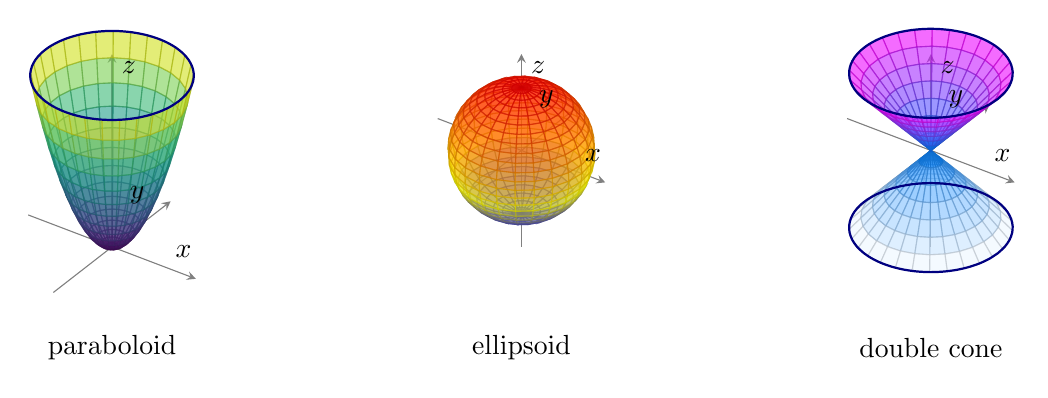
\begin{tikzpicture}[>=latex]

    % --- PARABOLOID ---
    \begin{axis}[
        name=paraboloid,
        view={35}{30},
        width=5.2cm, height=6cm,
        axis lines=center,
        axis line style={gray, thin},
        xlabel={\(x\)}, ylabel={\(y\)}, zlabel={\(z\)},
        ticks=none,
        xmin=-2.5, xmax=2.5,
        ymin=-2.5, ymax=2.5,
        zmin=0, zmax=4.5,
    ]
        % Main surface (r=x, theta=y)
        \addplot3[
            surf,
            colormap/viridis,
            opacity=0.6,
            samples=15,
            samples y=30,
            domain=0:2,
            domain y=0:360,
            z buffer=sort
        ] ({x*cos(y)}, {x*sin(y)}, {x^2});

        % Top rim edge
        \addplot3[
            smooth,
            blue!50!black, thick,
            domain=0:360,
            samples=40,
            samples y=0
        ] ({2*cos(x)}, {2*sin(x)}, {4});
    \end{axis}
    \node[align=center] at ([yshift=-0.3cm]paraboloid.south) {paraboloid};


    % --- ELLIPSOID ---
    \begin{axis}[
        name=ellipsoid,
        at={(5.2cm,0)},
        view={35}{30},
        width=5.2cm, height=6cm,
        axis lines=center,
        axis line style={gray, thin},
        xlabel={\(x\)}, ylabel={\(y\)}, zlabel={\(z\)},
        ticks=none,
        xmin=-2.5, xmax=2.5,
        ymin=-2.5, ymax=2.5,
        zmin=-2, zmax=2,
    ]
        % Main surface (theta=x, phi=y)
        \addplot3[
            surf,
            colormap/hot,
            opacity=0.6,
            samples=25,
            samples y=25,
            domain=0:360,
            domain y=0:180,
            z buffer=sort
        ] ({1.8*cos(x)*sin(y)}, {1.8*sin(x)*sin(y)}, {1.3*cos(y)});
    \end{axis}
    \node[align=center] at ([yshift=-0.3cm]ellipsoid.south) {ellipsoid};


    % --- DOUBLE CONE ---
    \begin{axis}[
        name=doublecone,
        at={(10.4cm,0)},
        view={35}{30},
        width=5.2cm, height=6cm,
        axis lines=center,
        axis line style={gray, thin},
        xlabel={\(x\)}, ylabel={\(y\)}, zlabel={\(z\)},
        ticks=none,
        xmin=-2.5, xmax=2.5,
        ymin=-2.5, ymax=2.5,
        zmin=-2.5, zmax=2.5,
    ]
        % Main surface (z=x, theta=y)
        \addplot3[
            surf,
            colormap/cool,
            opacity=0.6,
            samples=15,
            samples y=30,
            domain=-2:2,
            domain y=0:360,
            z buffer=sort
        ] ({x*cos(y)}, {x*sin(y)}, {x});

        % Top rim edge
        \addplot3[
            smooth,
            blue!50!black, thick,
            domain=0:360,
            samples=40,
            samples y=0
        ] ({2*cos(x)}, {2*sin(x)}, {2});

        % Bottom rim edge
        \addplot3[
            smooth,
            blue!50!black, thick,
            domain=0:360,
            samples=40,
            samples y=0
        ] ({2*cos(x)}, {2*sin(x)}, {-2});
    \end{axis}
    \node[align=center] at ([yshift=-0.3cm]doublecone.south) {double cone};

\end{tikzpicture}
\caption{Several common quadric surfaces can be recognized from their slices.}
\end{figure}

\subsection{Hyperboloids and saddle surfaces}

The signs in a quadric equation matter.  Positive square terms tend to make ellipses.
A mixture of positive and negative square terms tends to create hyperbolas.

\begin{example}[A hyperboloid of one sheet]
Consider
\[
    x^2+y^2-z^2=1.
\]
At \(z=0\), the horizontal slice is
\[
    x^2+y^2=1,
\]
a circle of radius \(1\).

At \(z=2\), the slice is
\[
    x^2+y^2-4=1,
\]
so
\[
    x^2+y^2=5,
\]
a larger circle.

At \(z=-2\), we get the same circle.

The surface is connected, with a narrow waist at \(z=0\).  It is called a
\emph{hyperboloid of one sheet}.
\end{example}

\begin{example}[A hyperboloid of two sheets]
Now change the signs:
\[
    z^2-x^2-y^2=1.
\]
At \(z=0\), the equation becomes
\[
    -x^2-y^2=1,
\]
which has no real solutions.

At \(z=2\), we get
\[
    4-x^2-y^2=1,
\]
so
\[
    x^2+y^2=3.
\]
At \(z=-2\), we get the same circle.

The surface has two disconnected pieces: one above and one below.  It is called a
\emph{hyperboloid of two sheets}.
\end{example}

The difference between
\[
    x^2+y^2-z^2=1
\]
and
\[
    z^2-x^2-y^2=1
\]
is not cosmetic.  It changes a connected surface into two separated pieces.

\begin{example}[A saddle surface]
The equation
\[
    z=x^2-y^2
\]
describes a \emph{hyperbolic paraboloid}, often called a saddle.

Look at two vertical slices.

If
\[
    y=0,
\]
then
\[
    z=x^2.
\]
This is an upward-opening parabola.

If
\[
    x=0,
\]
then
\[
    z=-y^2.
\]
This is a downward-opening parabola.

So in one direction the surface bends upward, while in the perpendicular direction it
bends downward.  That is the saddle shape.
\end{example}
\begin{figure}[h]
\centering
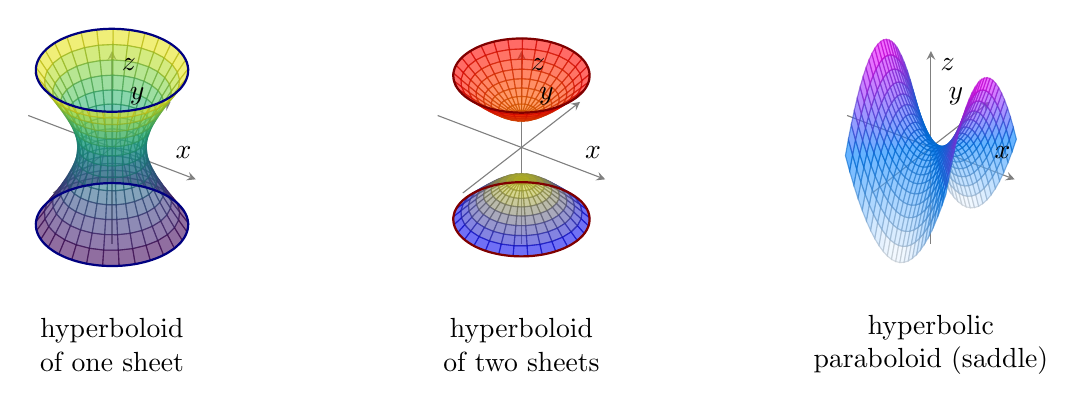
\begin{tikzpicture}[>=latex]

    % --- HYPERBOLOID OF ONE SHEET ---
    \begin{axis}[
        name=hyp1,
        view={35}{30},
        width=5.2cm, height=6cm,
        axis lines=center,
        axis line style={gray, thin},
        xlabel={\(x\)}, ylabel={\(y\)}, zlabel={\(z\)},
        ticks=none,
        xmin=-3, xmax=3, ymin=-3, ymax=3, zmin=-2.5, zmax=2.5,
    ]
        % Main surface (z=x, theta=y)
        \addplot3[
            surf,
            colormap/viridis,
            opacity=0.6,
            samples=15, samples y=30,
            domain=-2:2, domain y=0:360,
            z buffer=sort
        ] ({sqrt(1+x^2)*cos(y)}, {sqrt(1+x^2)*sin(y)}, {x});

        % Top rim edge
        \addplot3[smooth, blue!50!black, thick, domain=0:360, samples=40, samples y=0] 
            ({sqrt(5)*cos(x)}, {sqrt(5)*sin(x)}, {2});
        % Bottom rim edge
        \addplot3[smooth, blue!50!black, thick, domain=0:360, samples=40, samples y=0] 
            ({sqrt(5)*cos(x)}, {sqrt(5)*sin(x)}, {-2});
    \end{axis}
    \node[align=center] at ([yshift=-0.3cm]hyp1.south) {hyperboloid \\ of one sheet};


    % --- HYPERBOLOID OF TWO SHEETS ---
    \begin{axis}[
        name=hyp2,
        at={(5.2cm,0)},
        view={35}{30},
        width=5.2cm, height=6cm,
        axis lines=center,
        axis line style={gray, thin},
        xlabel={\(x\)}, ylabel={\(y\)}, zlabel={\(z\)},
        ticks=none,
        xmin=-3, xmax=3, ymin=-3, ymax=3, zmin=-3, zmax=3,
    ]
        % Top sheet (r=x, theta=y)
        \addplot3[
            surf,
            colormap/hot,
            opacity=0.6,
            samples=10, samples y=30,
            domain=0:2, domain y=0:360,
            z buffer=sort
        ] ({x*cos(y)}, {x*sin(y)}, {sqrt(1+x^2)});
        % Top rim edge
        \addplot3[smooth, red!50!black, thick, domain=0:360, samples=40, samples y=0] 
            ({2*cos(x)}, {2*sin(x)}, {sqrt(5)});

        % Bottom sheet
        \addplot3[
            surf,
            colormap/hot,
            opacity=0.6,
            samples=10, samples y=30,
            domain=0:2, domain y=0:360,
            z buffer=sort
        ] ({x*cos(y)}, {x*sin(y)}, {-sqrt(1+x^2)});
        % Bottom rim edge
        \addplot3[smooth, red!50!black, thick, domain=0:360, samples=40, samples y=0] 
            ({2*cos(x)}, {2*sin(x)}, {-sqrt(5)});
    \end{axis}
    \node[align=center] at ([yshift=-0.3cm]hyp2.south) {hyperboloid \\ of two sheets};


    % --- SADDLE (HYPERBOLIC PARABOLOID) ---
    \begin{axis}[
        name=saddle,
        at={(10.4cm,0)},
        view={35}{30},
        width=5.2cm, height=6cm,
        axis lines=center,
        axis line style={gray, thin},
        xlabel={\(x\)}, ylabel={\(y\)}, zlabel={\(z\)},
        ticks=none,
        xmin=-2.5, xmax=2.5, ymin=-2.5, ymax=2.5, zmin=-2.5, zmax=2.5,
    ]
        % Main Cartesian surface
        \addplot3[
            surf,
            colormap/cool,
            opacity=0.6,
            samples=25, samples y=25,
            domain=-1.5:1.5, domain y=-1.5:1.5,
            z buffer=sort
        ] {x^2 - y^2};
    \end{axis}
    \node[align=center] at ([yshift=-0.3cm]saddle.south) {hyperbolic \\ paraboloid (saddle)};

\end{tikzpicture}
\caption{Three surfaces defined by equations with mixed signs.}
\end{figure}
\begin{figure}[h]
\centering
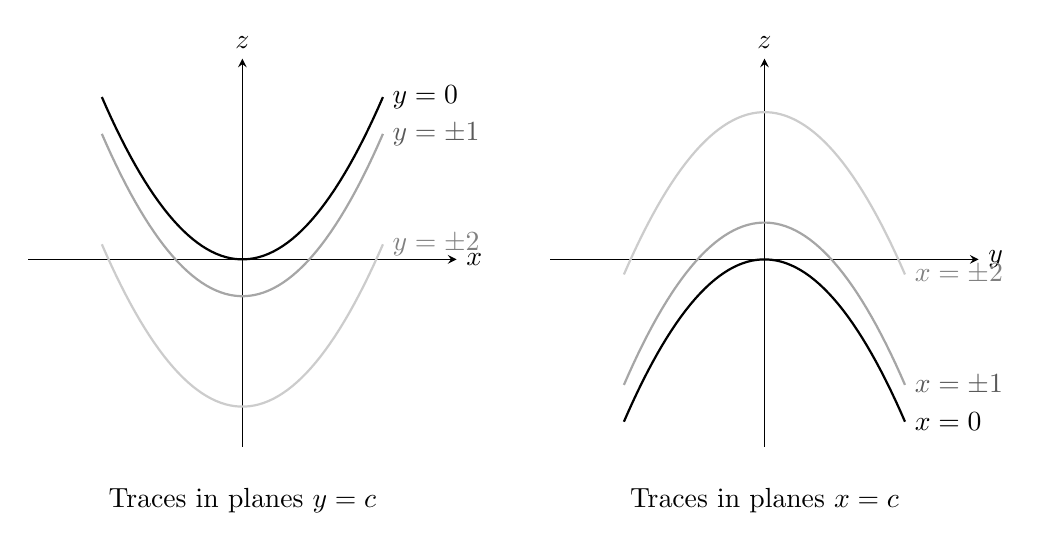
\begin{tikzpicture}[scale=0.85, >=stealth]

    % --- LEFT: Traces y=c ---
    \begin{scope}
        \draw[->] (-3.2,0) -- (3.2,0) node[right] {\(x\)};
        \draw[->] (0,-2.8) -- (0,3.0) node[above] {\(z\)};

        % y = \pm 2
        \draw[thick, gray!40, domain=-2.1:2.1, samples=60, variable=\x]
            plot ({\x},{0.55*\x*\x - 2.2});
        \node[right, gray] at (2.1, 0.22) {\(y=\pm 2\)};

        % y = \pm 1
        \draw[thick, gray!70, domain=-2.1:2.1, samples=60, variable=\x]
            plot ({\x},{0.55*\x*\x - 0.55});
        \node[right, gray!70!black] at (2.1, 1.87) {\(y=\pm 1\)};

        % y = 0
        \draw[thick, black, domain=-2.1:2.1, samples=60, variable=\x]
            plot ({\x},{0.55*\x*\x});
        \node[right] at (2.1, 2.42) {\(y=0\)};
        
        \node at (0, -3.6) {Traces in planes \(y=c\)};
    \end{scope}

    % --- RIGHT: Traces x=c ---
    \begin{scope}[shift={(7.8,0)}]
        \draw[->] (-3.2,0) -- (3.2,0) node[right] {\(y\)};
        \draw[->] (0,-2.8) -- (0,3.0) node[above] {\(z\)};

        % x = \pm 2
        \draw[thick, gray!40, domain=-2.1:2.1, samples=60, variable=\y]
            plot ({\y},{2.2 - 0.55*\y*\y});
        \node[right, gray] at (2.1, -0.22) {\(x=\pm 2\)};

        % x = \pm 1
        \draw[thick, gray!70, domain=-2.1:2.1, samples=60, variable=\y]
            plot ({\y},{0.55 - 0.55*\y*\y});
        \node[right, gray!70!black] at (2.1, -1.87) {\(x=\pm 1\)};

        % x = 0
        \draw[thick, black, domain=-2.1:2.1, samples=60, variable=\y]
            plot ({\y},{-0.55*\y*\y});
        \node[right] at (2.1, -2.42) {\(x=0\)};
        
        \node at (0, -3.6) {Traces in planes \(x=c\)};
    \end{scope}

\end{tikzpicture}
\caption{Families of traces for the saddle surface \(z=x^2-y^2\).}
\end{figure}

A saddle is one of the most important shapes in multivariable calculus.  Later, when
we study optimization, saddle points will be the places where a surface is level to first
order but is neither a maximum nor a minimum.

\subsection{Traces and cross-sections}

A \emph{trace} is a slice of a surface by a coordinate plane or by a plane parallel to a
coordinate plane.

The basic method is simple:

\[
\begin{array}{l}
\text{Set one coordinate equal to a constant.}\\
\text{Simplify the equation.}\\
\text{Recognize the curve left in the slice.}
\end{array}
\]

\begin{example}[Traces of an ellipsoid]
Consider
\[
    \frac{x^2}{9}+\frac{y^2}{4}+z^2=1.
\]
Horizontal traces come from fixing \(z\).

If
\[
    z=0,
\]
then
\[
    \frac{x^2}{9}+\frac{y^2}{4}=1.
\]
This is an ellipse.

If
\[
    z=\frac12,
\]
then
\[
    \frac{x^2}{9}+\frac{y^2}{4}+\frac14=1,
\]
so
\[
    \frac{x^2}{9}+\frac{y^2}{4}=\frac34.
\]
This is a smaller ellipse.

If
\[
    z=1,
\]
then
\[
    \frac{x^2}{9}+\frac{y^2}{4}=0,
\]
so the slice is only the point
\[
    (0,0,1).
\]
If
\[
    |z|>1,
\]
there are no points.

These slices tell us that the ellipsoid is widest at the middle and closes at the top and
bottom.
\end{example}

\begin{example}[Identifying a surface from traces]
Identify the surface
\[
    z=9-x^2-4y^2.
\]
Fix \(z=c\).  Then
\[
    c=9-x^2-4y^2,
\]
so
\[
    x^2+4y^2=9-c.
\]
For
\[
    c<9,
\]
this is an ellipse.  For
\[
    c=9,
\]
it is a single point.  For
\[
    c>9,
\]
there are no points.

So the surface has elliptical horizontal slices, with the largest slices lower down and
a top point at
\[
    (0,0,9).
\]
It is an elliptic paraboloid opening downward.
\end{example}

The same surface can often be recognized in several ways.  For
\[
    z=9-x^2-4y^2,
\]
fixing \(y=0\) gives
\[
    z=9-x^2,
\]
a downward-opening parabola.  Fixing \(x=0\) gives
\[
    z=9-4y^2,
\]
another downward-opening parabola, steeper in the \(y\)-direction.

That extra steepness is visible in the coefficient \(4\).

\subsection{A small gallery of standard quadric surfaces}

The following table is not meant to replace slicing.  It is a quick reference after slicing
has shown where the shapes come from.

\[
\begin{array}{c|c}
\text{Equation} & \text{Surface} \\ \hline
x^2+y^2=a^2 & \text{circular cylinder along the }z\text{-axis}\\[1mm]
z=x^2+y^2 & \text{elliptic paraboloid opening upward}\\[1mm]
z=-(x^2+y^2) & \text{elliptic paraboloid opening downward}\\[1mm]
z=x^2-y^2 & \text{hyperbolic paraboloid, or saddle}\\[1mm]
\dfrac{x^2}{a^2}+\dfrac{y^2}{b^2}+\dfrac{z^2}{c^2}=1
& \text{ellipsoid}\\[4mm]
x^2+y^2-z^2=1 & \text{hyperboloid of one sheet}\\[1mm]
z^2-x^2-y^2=1 & \text{hyperboloid of two sheets}\\[1mm]
z^2=x^2+y^2 & \text{double cone}
\end{array}
\]

A coefficient changes the stretching.  A sign changes the shape.  A missing variable
usually means a cylinder.  A shifted expression, such as
\[
    (x-2)^2+y^2+z^2=9,
\]
moves the surface away from the origin.

\begin{example}[A shifted sphere]
The equation
\[
    (x-2)^2+(y+1)^2+(z-3)^2=16
\]
is a sphere of radius \(4\), centered at
\[
    (2,-1,3).
\]
The shifted terms tell us the center:
\[
    x-2,\qquad y+1=y-(-1),\qquad z-3.
\]
\end{example}

\subsection{Level surfaces as three-dimensional contour maps}

A topographic map of a mountain uses level curves:
\[
    h(x,y)=c.
\]
Each curve connects points with the same elevation.

In space, a function
\[
    F(x,y,z)
\]
can have level surfaces:
\[
    F(x,y,z)=c.
\]
Each surface connects points where \(F\) has the same value.

\begin{definition}[Level surface]
Let
\[
    F:\mathbb R^3\to\mathbb R
\]
be a scalar-valued function.  A \emph{level surface} of \(F\) is a set of the form
\[
    F(x,y,z)=c,
\]
where \(c\) is a constant.
\end{definition}

\begin{example}[Temperature around a hot source]
Suppose the temperature near a small heater at the origin is modeled by
\[
    T(x,y,z)=\frac{100}{1+x^2+y^2+z^2}.
\]
The temperature depends only on distance from the origin.

The level surface where
\[
    T=20
\]
satisfies
\[
    \frac{100}{1+x^2+y^2+z^2}=20.
\]
So
\[
    1+x^2+y^2+z^2=5,
\]
and therefore
\[
    x^2+y^2+z^2=4.
\]
This is a sphere of radius \(2\).

So all points at distance \(2\) from the heater have the same temperature \(20\).
\end{example}

\begin{example}[Distance from the \(z\)-axis]
Let
\[
    F(x,y,z)=x^2+y^2.
\]
Then the level surface
\[
    F(x,y,z)=9
\]
is
\[
    x^2+y^2=9.
\]
This is a cylinder of radius \(3\) around the \(z\)-axis.

The function \(F\) measures squared distance from the \(z\)-axis, so its level surfaces
are cylinders.
\end{example}

Level surfaces are not just a way to draw shapes.  They are a way to understand scalar
fields in space: temperature, pressure, density, electric potential, gravitational potential,
and many others.

Later, when derivatives enter, a new vector will appear:
\[
    \nabla F.
\]
It will point perpendicular to the level surfaces of \(F\).  For now, the important point is
simpler: an equation
\[
    F(x,y,z)=c
\]
cuts space into surfaces of equal value.

\subsection{Equations describe surfaces, but not how to move on them}

An equation like
\[
    x^2+y^2+z^2=9
\]
tells us which points lie on a sphere.  But it does not tell us how to draw a grid on the
sphere.  It does not tell us how to walk across it using two parameters.  It does not tell
us, at least not directly, how a tiny patch of the surface should be measured.

For that, we need another description.  Instead of saying which points satisfy an equation,
we will build the surface from two moving parameters:
\[
    \mathbf r(u,v).
\]
A curve was a moving point.  A surface will be a moving curve, or equivalently, a point
that depends on two inputs.  That extra parameter is the doorway to tangent planes,
surface area, flux, and eventually the surface integrals where \(2\)-forms will do their
work.
\section{Parametric surfaces}
\label{sec:4.5}

Section \ref{sec:4.4} described surfaces by equations:
\[
    x^2+y^2+z^2=9,
    \qquad
    z=x^2-y^2,
    \qquad
    F(x,y,z)=c.
\]
An equation tells us which points belong to a surface.  But it does not tell us how to
walk on the surface, how to draw a grid on it, or how to measure a small tilted patch.

For that, we need parameters.

A curve used one parameter:
\[
    \mathbf r(t).
\]
A surface uses two:
\[
    \mathbf r(u,v).
\]
One parameter can move a point along a curve.  Two parameters can move a point across
a sheet.

\subsection{Surfaces as moving curves}

Start with a round pipe of radius \(2\) and height \(5\).  A point on the pipe can be
described by two choices:
\[
    \text{angle around the pipe},\qquad
    \text{height along the pipe}.
\]
Let the angle be \(\theta\) and the height be \(z\).  Then
\[
    \mathbf r(\theta,z)
    =
    (2\cos\theta,2\sin\theta,z),
    \qquad
    0\le \theta\le2\pi,\quad 0\le z\le5.
\]

If we hold \(z\) fixed, the point moves around a circle:
\[
    \theta\mapsto (2\cos\theta,2\sin\theta,z).
\]
If we hold \(\theta\) fixed, the point moves up a vertical line:
\[
    z\mapsto (2\cos\theta,2\sin\theta,z).
\]
The surface is made by letting both motions happen.

\begin{figure}[h]
\centering
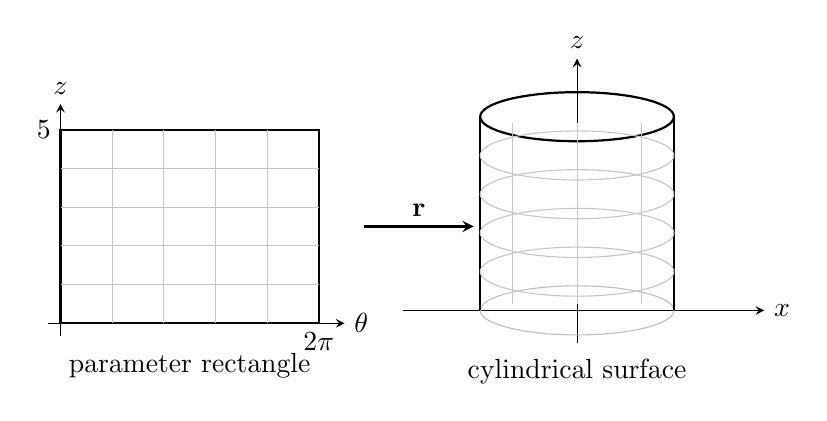
\begin{tikzpicture}[scale=0.82, >=stealth]
    % parameter domain
    \begin{scope}
        \draw[->] (-0.2,0) -- (4.4,0) node[right] {\(\theta\)};
        \draw[->] (0,-0.2) -- (0,3.4) node[above] {\(z\)};

        \draw[thick] (0,0) rectangle (4,3);

        \foreach \x in {0.8,1.6,2.4,3.2}
            \draw[gray!45] (\x,0) -- (\x,3);
        \foreach \y in {0.6,1.2,1.8,2.4}
            \draw[gray!45] (0,\y) -- (4,\y);

        \node at (2,-0.65) {parameter rectangle};
        \node[left] at (0,3) {\(5\)};
        \node[below] at (4,0) {\(2\pi\)};
    \end{scope}

    % arrow
    \draw[->, thick] (4.7,1.5) -- (6.4,1.5) node[midway, above] {\(\mathbf r\)};

    % cylinder
    \begin{scope}[shift={(8,0.2)}]
        \draw[->] (-2.7,0) -- (2.9,0) node[right] {\(x\)};
        \draw[->] (0,-0.5) -- (0,3.9) node[above] {\(z\)};

        \draw[gray!50] (0,0) ellipse (1.5 and 0.38);
        \draw[thick] (-1.5,0) -- (-1.5,3);
        \draw[thick] (1.5,0) -- (1.5,3);
        \draw[thick] (0,3) ellipse (1.5 and 0.38);

        \foreach \h in {0.6,1.2,1.8,2.4}
            \draw[gray!45] (0,\h) ellipse (1.5 and 0.38);

        \foreach \x in {-1.0,0,1.0}
            \draw[gray!45] (\x,0.1) -- (\x,2.9);

        \node at (0,-0.95) {cylindrical surface};
    \end{scope}
\end{tikzpicture}
\caption{The rectangle of parameter values is wrapped into a cylinder.}
\end{figure}

\begin{definition}[Parametrized surface]
A \emph{parametrized surface} in \(\mathbb R^3\) is a continuous function
\[
    \mathbf r:D\to\mathbb R^3,
\]
where \(D\) is a region in the \(uv\)-plane.  We write
\[
    \mathbf r(u,v)=\bigl(x(u,v),y(u,v),z(u,v)\bigr).
\]
The \emph{image} of the parametrization is the set of points
\[
    \{\mathbf r(u,v):(u,v)\in D\}.
\]
\end{definition}

The region \(D\) is called the \emph{parameter domain}.  It might be a rectangle, a
disk, a triangle, or some other region.

We often use the same phrase ``parametric surface'' for both the map
\[
    \mathbf r(u,v)
\]
and the geometric surface it traces.  When the distinction matters, we will say
\emph{parametrization} for the map and \emph{surface} for the image.

The continuity condition matters for the same reason it mattered for curves.  A surface
should not tear or teleport.

\begin{example}[A discontinuous rule is not a sheet]
Define
\[
    \mathbf r(u,v)=
    \begin{cases}
    (u,v,0), & u<0,\\
    (u,v,1), & u\ge0,
    \end{cases}
\]
on the square
\[
    -1\le u\le1,\qquad -1\le v\le1.
\]
The left half of the square is sent to the plane \(z=0\), while the right half is sent to
the plane \(z=1\).  Along \(u=0\), the image jumps upward by one unit.

This is not one continuous surface patch.  It is two half-sheets separated by a tear.
\end{example}

\subsection{Graphs as parametrized surfaces}

Every graph
\[
    z=f(x,y)
\]
has a natural parametrization:
\[
    \mathbf r(u,v)=(u,v,f(u,v)).
\]
The parameters are just the input coordinates.

\begin{example}[A bowl as a parametrized surface]
Consider the elliptic bowl
\[
    z=4-\frac{x^2}{9}-\frac{y^2}{4}.
\]
Using
\[
    x=u,\qquad y=v,
\]
we get
\[
    \mathbf r(u,v)
    =
    \left(
        u,\,
        v,\,
        4-\frac{u^2}{9}-\frac{v^2}{4}
    \right).
\]
If we use all pairs \((u,v)\), this traces the whole paraboloid.  If we restrict the
domain, for example to
\[
    -3\le u\le3,\qquad -2\le v\le2,
\]
we get only a rectangular patch of the bowl.
\end{example}

This is one reason parametrizations are useful.  The same formula can describe a whole
surface or only a chosen piece of it, depending on the parameter domain.

A plane from Chapter 1 is also a parametrized surface:
\[
    \mathbf r(u,v)=P+u\mathbf a+v\mathbf b.
\]
The two parameters say how far to move in the two plane directions.

\begin{example}[An affine plane as a parametrized surface]
Let
\[
    P=(1,0,2),\qquad \mathbf a=(2,1,0),\qquad \mathbf b=(0,1,3).
\]
Then
\[
    \mathbf r(u,v)
    =
    (1,0,2)+u(2,1,0)+v(0,1,3).
\]
So
\[
    \mathbf r(u,v)=(1+2u,\;u+v,\;2+3v).
\]
This is the plane through \(P\) spanned by the directions \(\mathbf a\) and
\(\mathbf b\).
\end{example}

The formula
\[
    P+u\mathbf a+v\mathbf b
\]
is the flat version of a surface.  A general parametrized surface is what happens when
the two directions are allowed to bend as we move.

\subsection{Coordinate grids on surfaces}

A parametrization does more than trace points.  It brings a grid with it.

For a surface
\[
    \mathbf r(u,v),
\]
there are two natural families of curves.

If we hold \(u=u_0\) fixed, we get the curve
\[
    v\mapsto \mathbf r(u_0,v).
\]
If we hold \(v=v_0\) fixed, we get the curve
\[
    u\mapsto \mathbf r(u,v_0).
\]
These are called \emph{coordinate curves} or \emph{grid curves}.

\begin{definition}[Grid curves on a parametrized surface]
For a parametrized surface
\[
    \mathbf r(u,v),
\]
the curves
\[
    \mathbf r(u_0,v)
\]
and
\[
    \mathbf r(u,v_0)
\]
are called the \emph{grid curves} of the parametrization.
\end{definition}

On the cylinder
\[
    \mathbf r(\theta,z)=(2\cos\theta,2\sin\theta,z),
\]
the grid curves are easy to see.

Holding \(z\) fixed gives horizontal circles.  Holding \(\theta\) fixed gives vertical
lines.

On a sphere, the same idea becomes latitude and longitude.

\begin{example}[Latitude and longitude as grid curves]
The sphere of radius \(3\) can be parametrized by
\[
    \mathbf r(\theta,\phi)
    =
    (3\sin\phi\cos\theta,\,
     3\sin\phi\sin\theta,\,
     3\cos\phi),
\]
where
\[
    0\le\theta\le2\pi,\qquad 0\le\phi\le\pi.
\]
Here \(\theta\) goes around the \(z\)-axis, and \(\phi\) measures angle down from the
positive \(z\)-axis.

If \(\phi\) is fixed, then
\[
    z=3\cos\phi
\]
is fixed, and the point moves around a circle of latitude.

If \(\theta\) is fixed, then the point moves along a meridian from the north pole to the
south pole.
\end{example}

This parametrization also shows a small warning.  At
\[
    \phi=0
\]
all values of \(\theta\) give the same point:
\[
    (0,0,3).
\]
At
\[
    \phi=\pi,
\]
all values of \(\theta\) give
\[
    (0,0,-3).
\]
Also, \(\theta=0\) and \(\theta=2\pi\) trace the same meridian.  So the parametrization
is not one-to-one on the full parameter rectangle.

That is not a mistake.  Many useful parametrizations repeat some points.  The important
thing is to notice when it happens.

\subsection{Tangent directions from parameter curves}

A parametrization gives us two grid curves through most points.  Each grid curve has
a tangent direction.

For
\[
    \mathbf r(u,v),
\]
we define
\[
    \mathbf r_u
\]
by holding \(v\) fixed and differentiating with respect to \(u\).  We define
\[
    \mathbf r_v
\]
by holding \(u\) fixed and differentiating with respect to \(v\).

This notation will become more systematic when we study partial derivatives.  For now,
it is only single-variable calculus applied to the two parameter curves.

\begin{example}[Tangent directions on a cylinder]
For the cylinder
\[
    \mathbf r(\theta,z)=(2\cos\theta,2\sin\theta,z),
\]
differentiate with respect to \(\theta\):
\[
    \mathbf r_\theta(\theta,z)=(-2\sin\theta,2\cos\theta,0).
\]
This points around the cylinder.

Differentiate with respect to \(z\):
\[
    \mathbf r_z(\theta,z)=(0,0,1).
\]
This points straight upward.

At
\[
    \theta=\frac{\pi}{3},\qquad z=2,
\]
the point on the cylinder is
\[
    \mathbf r\left(\frac{\pi}{3},2\right)
    =
    (1,\sqrt3,2).
\]
The two tangent directions are
\[
    \mathbf r_\theta\left(\frac{\pi}{3},2\right)
    =
    (-\sqrt3,1,0)
\]
and
\[
    \mathbf r_z\left(\frac{\pi}{3},2\right)
    =
    (0,0,1).
\]
One direction goes around the pipe.  The other goes up the pipe.
\end{example}

\begin{figure}[h]
\centering
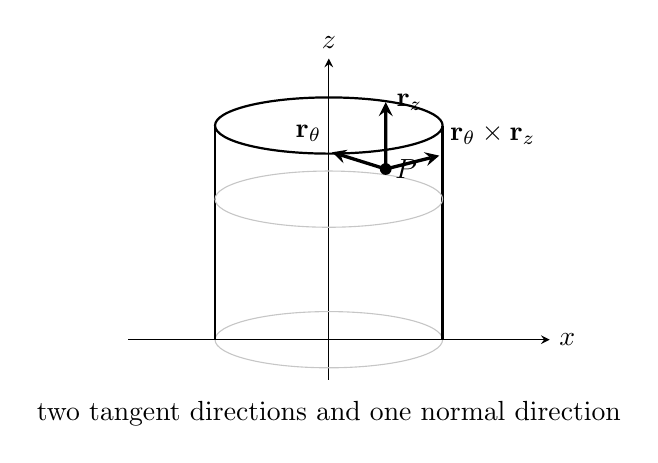
\begin{tikzpicture}[scale=0.85, >=stealth]
    % cylinder sketch
    \draw[->] (-3,0) -- (3.3,0) node[right] {\(x\)};
    \draw[->] (0,-0.6) -- (0,4.2) node[above] {\(z\)};

    \draw[gray!45] (0,0) ellipse (1.7 and 0.42);
    \draw[thick] (-1.7,0) -- (-1.7,3.2);
    \draw[thick] (1.7,0) -- (1.7,3.2);
    \draw[thick] (0,3.2) ellipse (1.7 and 0.42);

    \draw[gray!45] (0,2.1) ellipse (1.7 and 0.42);

    \coordinate (P) at (0.85,2.55);
    \fill (P) circle (2.5pt);
    \node[right] at (P) {\(P\)};

    \draw[->, very thick] (P) -- (0.05,2.8) node[above left] {\(\mathbf r_\theta\)};
    \draw[->, very thick] (P) -- (0.85,3.55) node[right] {\(\mathbf r_z\)};
    \draw[->, very thick] (P) -- (1.65,2.75) node[above right] {\(\mathbf r_\theta\times\mathbf r_z\)};

    \node at (0,-1.1) {two tangent directions and one normal direction};
\end{tikzpicture}
\caption{The two parameter directions on a cylinder give two tangent directions.}
\end{figure}

The two tangent directions often span the tangent plane to the surface.  But this only
works when they are genuinely two different directions.

\begin{definition}[Regular point of a parametrized surface]
Suppose the derivatives
\[
    \mathbf r_u(u_0,v_0),
    \qquad
    \mathbf r_v(u_0,v_0)
\]
exist.  The parametrization is called \emph{regular} at \((u_0,v_0)\) if
\[
    \mathbf r_u(u_0,v_0)\times \mathbf r_v(u_0,v_0)\neq \mathbf 0.
\]
Equivalently, the two tangent directions are not parallel and neither has collapsed
enough to make the parallelogram have zero area.
\end{definition}

This condition is not just technical language.  It tells us when the parameters really
make a two-dimensional patch.

\begin{example}[Why regularity matters: the tip of a cone]
The upper cone
\[
    z=\sqrt{x^2+y^2}
\]
has the parametrization
\[
    \mathbf r(s,\theta)
    =
    (s\cos\theta,s\sin\theta,s),
    \qquad
    s\ge0,\quad 0\le\theta\le2\pi.
\]
For \(s>0\), the parameters describe points away from the tip.

At the tip,
\[
    s=0,
\]
all angles give the same point:
\[
    \mathbf r(0,\theta)=(0,0,0).
\]
The tangent directions are
\[
    \mathbf r_s=(\cos\theta,\sin\theta,1),
\]
and
\[
    \mathbf r_\theta=(-s\sin\theta,s\cos\theta,0).
\]
At \(s=0\),
\[
    \mathbf r_\theta=(0,0,0).
\]
So
\[
    \mathbf r_s\times\mathbf r_\theta=\mathbf 0.
\]
The parametrization is not regular at the tip.

Geometrically, this matches what we see.  The cone has a sharp point.  There is no
single tangent plane there.
\end{example}

So a parametrization may still describe a surface even at a nonregular point, but the
calculus we want later needs regular points.  Surface area, flux, and tangent planes all
depend on small surface patches behaving like small parallelograms.

\subsection{Orientation preview: choosing a side of a surface}

Recall from Chapter 2 that the order of two vectors matters for signed area:
\[
    \mathbf a\wedge\mathbf b=-\mathbf b\wedge\mathbf a.
\]
The same sign issue appears on surfaces.

For the cylinder
\[
    \mathbf r(\theta,z)=(2\cos\theta,2\sin\theta,z),
\]
we computed
\[
    \mathbf r_\theta=(-2\sin\theta,2\cos\theta,0),
    \qquad
    \mathbf r_z=(0,0,1).
\]
Their cross product is
\[
\begin{aligned}
    \mathbf r_\theta\times \mathbf r_z
    &=
    (2\cos\theta,2\sin\theta,0).
\end{aligned}
\]
This points outward from the cylinder.

But if we reverse the parameter order, using
\[
    \widetilde{\mathbf r}(z,\theta)=\mathbf r(\theta,z),
\]
then the corresponding normal is
\[
    \mathbf r_z\times\mathbf r_\theta
    =
    -(\mathbf r_\theta\times\mathbf r_z),
\]
which points inward.

Same cylinder.  Opposite orientation.

\begin{definition}[Orientation, informally]
An \emph{orientation} of a two-sided surface is a consistent choice of side, or
equivalently a consistent choice of normal direction.

For a parametrized patch, the order of the parameters gives an orientation through
\[
    \mathbf r_u\times\mathbf r_v.
\]
Reversing the parameter order reverses the orientation.
\end{definition}

This will matter later in exactly the same way orientation mattered for curves.  If we
walk around a closed curve in the opposite direction, a line integral changes sign.  If we
choose the opposite side of a surface, a flux integral changes sign.

In differential-form language, a small positive parameter patch
\[
    du\wedge dv
\]
is sent to an oriented patch on the surface.  Swapping the parameters changes
\[
    du\wedge dv
\]
to
\[
    dv\wedge du=-du\wedge dv.
\]
The sign is not decoration.  It records which side of the surface we have chosen.

Not every surface allows a consistent choice of side.  A M\"obius strip is the famous
warning: if you walk around it, a normal vector that began on one side returns on the
other side.  We will not need that example for most computations, but it explains why
orientation is something we choose carefully instead of assuming automatically.

A parametrized surface is therefore more than a picture.  It is a map from a flat
parameter region onto a possibly curved sheet.  It carries grid curves, tangent directions,
and an orientation.  Those are exactly the pieces that surface integrals will need later.

For now, Chapter 4 has done its job.  We can describe curves, coordinates, surfaces,
and parameter grids before differentiating or integrating them seriously.  The next page
collects those tools.  After that, the first parameter becomes time again, and a curve
starts moving.

\section{Chapter review and visual projects}
\label{sec:4.6}

Chapter 4 began with a moving point
\[
    \mathbf r(t),
\]
then widened the language of coordinates and surfaces.  We learned that the same
geometric object can have several descriptions: an equation, a coordinate condition, a
level surface, or a parametrization.

The skill is not to memorize one favorite description.  The skill is to choose the one
that makes the geometry speak clearly.

\subsection{The chapter in one picture}

\[
\begin{array}{c|c|c}
\text{Object} & \text{Typical description} & \text{What it emphasizes} \\ \hline
\text{parametric curve} &
\mathbf r(t)=(x(t),y(t),z(t)) &
\text{motion along a path}\\[1mm]
\text{polar curve} &
r=f(\theta) &
\text{distance and angle in the plane}\\[1mm]
\text{cylindrical surface} &
r=a,\ z=f(r,\theta) &
\text{distance from an axis}\\[1mm]
\text{spherical surface} &
\rho=a,\ \phi=\text{constant} &
\text{distance and angles from a center}\\[1mm]
\text{quadric surface} &
\text{second-degree equation} &
\text{slices and traces}\\[1mm]
\text{level surface} &
F(x,y,z)=c &
\text{equal values of a scalar field}\\[1mm]
\text{parametric surface} &
\mathbf r(u,v) &
\text{a grid drawn on a surface}
\end{array}
\]

A surface like a sphere may appear in many rows of this table:
\[
    x^2+y^2+z^2=a^2,
\]
\[
    \rho=a,
\]
or
\[
    \mathbf r(\theta,\phi)
    =
    (a\sin\phi\cos\theta,\,
     a\sin\phi\sin\theta,\,
     a\cos\phi).
\]
Each description sees a different part of the same geometry.

\subsection{Skills: converting coordinates and recognizing surfaces}

By the end of this chapter, the following moves should feel familiar.

\subsubsection*{Coordinate conversions}

\[
\begin{array}{c|c}
\text{System} & \text{Conversion to rectangular coordinates} \\ \hline
\text{polar} &
x=r\cos\theta,\quad y=r\sin\theta\\[1mm]
\text{cylindrical} &
x=r\cos\theta,\quad y=r\sin\theta,\quad z=z\\[1mm]
\text{spherical} &
x=\rho\sin\phi\cos\theta,\quad
y=\rho\sin\phi\sin\theta,\quad
z=\rho\cos\phi
\end{array}
\]

The distance formulas are
\[
    r^2=x^2+y^2
\]
and
\[
    \rho^2=x^2+y^2+z^2.
\]

The angle formulas need quadrant care:
\[
    \tan\theta=\frac{y}{x}
\]
does not by itself determine \(\theta\).

\subsubsection*{Surface recognition}

A missing variable often means a cylinder.  For example,
\[
    x^2+y^2=9
\]
in space is a cylinder, because \(z\) is free.

A squared-distance equation usually points toward a sphere or ellipsoid:
\[
    x^2+y^2+z^2=25
\]
is a sphere, while
\[
    \frac{x^2}{9}+\frac{y^2}{4}+z^2=1
\]
is an ellipsoid.

A variable equal to a sum of squares usually gives a paraboloid:
\[
    z=x^2+4y^2
\]
opens upward, while
\[
    z=9-x^2-4y^2
\]
opens downward.

Mixed signs create hyperbolic behavior:
\[
    x^2+y^2-z^2=1
\]
is a hyperboloid of one sheet, while
\[
    z^2-x^2-y^2=1
\]
is a hyperboloid of two sheets.

A difference of squares in a graph gives a saddle:
\[
    z=x^2-y^2.
\]

\subsubsection*{Slicing strategy}

To understand a surface, slice it.

\[
\begin{array}{l}
\text{Fix }z=c\text{ for horizontal traces.}\\
\text{Fix }x=c\text{ or }y=c\text{ for vertical traces.}\\
\text{Simplify the remaining equation.}\\
\text{Recognize the curve in the slice.}
\end{array}
\]

\begin{example}[A review identification]
Identify
\[
    4x^2+y^2+z^2=16.
\]
Divide by \(16\):
\[
    \frac{x^2}{4}+\frac{y^2}{16}+\frac{z^2}{16}=1.
\]
This is an ellipsoid.  It reaches
\[
    x=\pm2,\qquad y=\pm4,\qquad z=\pm4.
\]
So it is shorter in the \(x\)-direction than in the \(y\)- and \(z\)-directions.
\end{example}

\begin{example}[A review parametrization]
Parametrize the upper cone
\[
    z=2\sqrt{x^2+y^2}.
\]
Use cylindrical coordinates:
\[
    x=r\cos\theta,\qquad y=r\sin\theta,\qquad z=2r.
\]
So
\[
    \mathbf r(r,\theta)
    =
    (r\cos\theta,r\sin\theta,2r),
    \qquad
    r\ge0,\quad 0\le\theta\le2\pi.
\]
If we only want the part below \(z=6\), then
\[
    2r\le6,
\]
so
\[
    0\le r\le3.
\]
\end{example}

\subsection{Practice problems}

\subsubsection*{A. Parametric curves and polar coordinates}

\begin{enumerate}
\item Sketch the curve
\[
    \mathbf r(t)=(2\cos t,2\sin t),
    \qquad 0\le t\le\pi.
\]
State its orientation.

\item The curve
\[
    \mathbf r(t)=(\cos 2t,\sin 2t),
    \qquad 0\le t\le2\pi,
\]
traces the unit circle how many times?

\item Convert the polar point
\[
    \left(6,\frac{5\pi}{6}\right)
\]
to Cartesian coordinates.

\item Convert the Cartesian point
\[
    (2,-2)
\]
to polar coordinates with \(r>0\) and \(0\le\theta<2\pi\).

\item Identify the polar graph
\[
    r=5.
\]

\item Convert
\[
    r=6\sin\theta
\]
to a Cartesian equation and identify the curve.
\end{enumerate}

\subsubsection*{B. Cylindrical and spherical coordinates}

\begin{enumerate}
\item Convert
\[
    (r,\theta,z)=\left(4,\frac{\pi}{3},2\right)
\]
to rectangular coordinates.

\item Convert
\[
    (x,y,z)=(-1,\sqrt3,5)
\]
to cylindrical coordinates.

\item Convert the spherical point
\[
    \left(\rho,\theta,\phi\right)
    =
    \left(3,\frac{\pi}{4},\frac{\pi}{3}\right)
\]
to rectangular coordinates.

\item Describe the cylindrical surface
\[
    r=2.
\]

\item Describe the spherical surface
\[
    \rho=4.
\]

\item Describe the spherical surface
\[
    \phi=\frac{\pi}{6}.
\]
\end{enumerate}

\subsubsection*{C. Quadric and level surfaces}

\begin{enumerate}
\item Identify the surface
\[
    x^2+y^2=16.
\]

\item Identify the surface
\[
    z=x^2+3y^2.
\]

\item Identify the surface
\[
    \frac{x^2}{4}+\frac{y^2}{9}+\frac{z^2}{25}=1.
\]

\item Identify the surface
\[
    x^2+y^2-z^2=4.
\]

\item Identify the surface
\[
    z=x^2-y^2.
\]

\item The temperature in a room is modeled by
\[
    T(x,y,z)=20+x^2+y^2+z^2.
\]
Describe the level surface
\[
    T=29.
\]
\end{enumerate}

\subsubsection*{D. Parametric surfaces}

\begin{enumerate}
\item Identify the surface
\[
    \mathbf r(u,v)=(u,v,u^2+v^2).
\]

\item Identify the surface
\[
    \mathbf r(\theta,z)=(3\cos\theta,3\sin\theta,z).
\]

\item Find a parametrization of the plane through
\[
    P=(1,2,3)
\]
with direction vectors
\[
    \mathbf a=(1,0,1),
    \qquad
    \mathbf b=(0,2,-1).
\]

\item Find a parametrization of the sphere
\[
    x^2+y^2+z^2=9.
\]

\item For
\[
    \mathbf r(u,v)=(u,v,uv),
\]
describe the two families of grid curves:
\[
    u=\text{constant}
    \qquad\text{and}\qquad
    v=\text{constant}.
\]

\item For
\[
    \mathbf r(\theta,z)=(2\cos\theta,2\sin\theta,z),
\]
compute
\[
    \mathbf r_\theta\times\mathbf r_z.
\]
Does it point inward or outward?
\end{enumerate}

\subsection{Project: build a gallery of quadrics}

Create a visual gallery of the main quadric surfaces from Section \ref{sec:4.4}.

For each surface, include:

\[
\begin{array}{ll}
1. & \text{the equation,}\\
2. & \text{three traces or cross-sections,}\\
3. & \text{a hand sketch or computer-generated plot,}\\
4. & \text{one sentence explaining how the signs and coefficients shape it.}
\end{array}
\]

Use at least six of the following:

\[
\begin{array}{c}
x^2+y^2=4,\\[1mm]
z=x^2+y^2,\\[1mm]
z=x^2-y^2,\\[1mm]
\dfrac{x^2}{9}+\dfrac{y^2}{4}+z^2=1,\\[4mm]
x^2+y^2-z^2=1,\\[1mm]
z^2-x^2-y^2=1,\\[1mm]
z^2=x^2+y^2,\\[1mm]
y=x^2.
\end{array}
\]

For the last equation,
\[
    y=x^2,
\]
remember that this is a surface in space, not just a plane parabola.  The missing
variable \(z\) is free.

A good gallery should not look like a list of formulas.  It should show how the formulas
turn into shapes.

\subsection{Project: compare several parametrizations of a sphere}

The sphere
\[
    x^2+y^2+z^2=a^2
\]
has many parametrizations.  Compare the following three.

\subsubsection*{1. Spherical-coordinate parametrization}

\[
    \mathbf r_1(\theta,\phi)
    =
    (a\sin\phi\cos\theta,\,
     a\sin\phi\sin\theta,\,
     a\cos\phi),
\]
where
\[
    0\le\theta\le2\pi,\qquad 0\le\phi\le\pi.
\]

\subsubsection*{2. Upper and lower graph parametrizations}

The upper hemisphere is
\[
    \mathbf r_2(u,v)
    =
    \left(u,v,\sqrt{a^2-u^2-v^2}\right),
    \qquad
    u^2+v^2\le a^2.
\]
The lower hemisphere is
\[
    \mathbf r_3(u,v)
    =
    \left(u,v,-\sqrt{a^2-u^2-v^2}\right),
    \qquad
    u^2+v^2\le a^2.
\]

\subsubsection*{3. Height-angle parametrization}

Use height \(z\) and angle \(\theta\):
\[
    \mathbf r_4(\theta,z)
    =
    \left(
        \sqrt{a^2-z^2}\cos\theta,\,
        \sqrt{a^2-z^2}\sin\theta,\,
        z
    \right),
\]
where
\[
    0\le\theta\le2\pi,\qquad -a\le z\le a.
\]

For each parametrization, answer:

\begin{enumerate}
\item What is the parameter domain?
\item Which parameter curves look like circles?
\item Which parameter curves run from pole to pole?
\item Where does the parametrization repeat points?
\item Where does the parametrization collapse a whole edge or curve to one point?
\item Which parametrization would you use to draw latitude and longitude?
\item Which would you use to describe the sphere as two graphs?
\end{enumerate}

This project is not only about spheres.  It teaches a larger lesson: a parametrization is
a choice of coordinates on a surface, and different choices reveal different geometry.

\subsection{A final hook: once curves move, velocity returns}

A curve can be described as a set of points, but a parametrized curve remembers how the
points are traced.  The circle
\[
    x^2+y^2=1
\]
does not know whether a particle moves clockwise or counterclockwise, quickly or
slowly, once or many times.  The parametrization
\[
    \mathbf r(t)=(\cos t,\sin t)
\]
does know.

That difference is about to become calculus again.  Once the parameter is time, a curve
has velocity.  Once velocity changes, it has acceleration.  The old single-variable idea
\[
    \text{rate of change}
\]
returns, but now the output is a vector and the path may bend through space.

The next chapter begins there: not with a new kind of surface, but with a moving point.